% =====================================================================
%  DocuMind AI — Final Year Project Report
%  COMSATS University Islamabad, Vehari Campus
%  Compile with pdflatex (Overleaf: Menu -> Compiler -> pdfLaTeX), twice
%  so that the table of contents and cross-references are filled in.
% =====================================================================
\documentclass[11pt,a4paper]{report}

% ---------- page and fonts ----------
\usepackage[a4paper,left=2cm,right=2cm,top=3cm,bottom=2.5cm]{geometry}
\usepackage[T1]{fontenc}
\usepackage[utf8]{inputenc}
\usepackage{lmodern}
\usepackage{microtype}
\usepackage{setspace}

% ---------- tables, lists, figures ----------
\usepackage{array}
\usepackage{tabularx}
\usepackage{longtable}
\usepackage{multirow}
\usepackage{makecell}
\usepackage{booktabs}
\usepackage[table]{xcolor}
\usepackage{enumitem}
\usepackage{graphicx}
\usepackage{float}
\usepackage[font=normalsize,skip=4pt]{caption}
\usepackage{amsmath,amssymb}
\usepackage{algorithm}
\usepackage{algpseudocode}
\usepackage{listings}
\usepackage{pifont}
\usepackage{adjustbox}

% ---------- diagrams ----------
\usepackage{tikz}
\usetikzlibrary{positioning,arrows.meta,shapes.geometric,shapes.multipart,shapes.misc,fit,calc,backgrounds}

% ---------- headings ----------
\usepackage{titlesec}
\titleformat{\chapter}[display]{\normalfont\LARGE\bfseries\centering}{\chaptertitlename\ \thechapter}{0pt}{\LARGE}
\titlespacing*{\chapter}{0pt}{20pt}{24pt}
\titleformat{name=\chapter,numberless}[display]{\normalfont\LARGE\bfseries\centering}{}{0pt}{\LARGE}
\setcounter{secnumdepth}{4}
\setcounter{tocdepth}{4}

\usepackage[hidelinks]{hyperref}

% ---------- spacing ----------
\setlength{\parskip}{2pt}
\setlength{\emergencystretch}{3em}
\setlist{itemsep=1pt,topsep=3pt}
\renewcommand{\arraystretch}{1.15}

% =====================================================================
%  Helper macros
% =====================================================================
\newcommand{\sysname}{DocuMind AI}
\newcommand{\code}[1]{\texttt{\small #1}}

% A visible marker for numbers that still have to be filled in.
\newcommand{\pending}[1]{\textcolor{red}{\textbf{[#1]}}}

% Screenshot: put the PNG in screens/ with the given name. Until then a framed
% placeholder with the same caption is printed, so the report always compiles.
\newcommand{\screenshot}[3]{%
  \begin{figure}[H]\centering
  \IfFileExists{screens/#1}{%
    \fbox{\includegraphics[width=0.92\textwidth,height=0.42\textheight,keepaspectratio]{screens/#1}}}{%
    \fbox{\parbox[c][5.5cm][c]{0.88\textwidth}{\centering\color{gray}\large
      Screenshot to insert:\\[4pt]\texttt{screens/#1}}}}
  \caption{#2}\label{#3}
  \end{figure}}

% TikZ figure from figures/<file>.tex, scaled down if it is larger than the page.
\newcommand{\tikzfig}[4][0.78]{%
  \begin{figure}[H]\centering
  \begin{adjustbox}{max width=\textwidth,max totalheight=#1\textheight}\input{figures/#2}\end{adjustbox}
  \caption{#3}\label{#4}
  \end{figure}}

% Two-column boxed table used for use cases and functional requirements.
\newenvironment{spec}[2]{%
  \begin{table}[H]\centering\caption{#1}\label{#2}
  \begin{tabular}{|>{\bfseries}p{3.4cm}|p{\dimexpr\textwidth-3.4cm-4\tabcolsep-3\arrayrulewidth\relax}|}\hline}{%
  \end{tabular}\end{table}}
\newcommand{\row}[2]{#1 & #2 \\ \hline}

% Compact numbered list inside table cells.
\newenvironment{steps}{\begin{minipage}[t]{\linewidth}\begin{enumerate}[leftmargin=*,nosep]}{\end{enumerate}\vspace{2pt}\end{minipage}}
\newenvironment{bullets}{\begin{minipage}[t]{\linewidth}\begin{itemize}[leftmargin=*,nosep]}{\end{itemize}\vspace{2pt}\end{minipage}}

% ---------- TikZ styles ----------
\tikzset{
  >={Stealth[length=2.2mm]},
  box/.style={draw,rounded corners=2pt,align=center,fill=white,font=\small,inner sep=4pt,minimum height=8mm},
  softbox/.style={box,fill=gray!8},
  tier/.style={draw,dashed,rounded corners=4pt,inner sep=8pt},
  tierlabel/.style={font=\small\bfseries,anchor=north west},
  db/.style={cylinder,shape border rotate=90,draw,aspect=0.18,align=center,font=\small,minimum width=24mm,minimum height=13mm,fill=white},
  act/.style={draw,rounded corners=7pt,align=center,font=\small,minimum height=7mm,inner sep=4pt,fill=white,text width=#1},
  act/.default=48mm,
  dec/.style={draw,diamond,aspect=2.4,align=center,font=\footnotesize,inner sep=1pt,fill=white},
  startnode/.style={circle,fill=black,minimum size=3.5mm,inner sep=0pt},
  endnode/.style={circle,draw,double,double distance=1.2pt,fill=black,minimum size=3mm,inner sep=0pt},
  flow/.style={->,thick},
  lbl/.style={font=\footnotesize,fill=white,inner sep=1.5pt},
  ent/.style={draw,rectangle split,rectangle split parts=2,align=left,font=\scriptsize,fill=white,inner sep=3pt,
              rectangle split part fill={gray!15,white}},
  usecase/.style={draw,ellipse,align=center,font=\footnotesize,minimum width=34mm,minimum height=8mm,inner sep=1pt,fill=white},
  state/.style={draw,rounded corners=8pt,align=center,font=\small,minimum height=8mm,minimum width=24mm,fill=white},
  proc/.style={draw,circle,align=center,font=\scriptsize,minimum size=19mm,inner sep=1pt,fill=white},
  extent/.style={draw,rectangle,align=center,font=\small,minimum height=9mm,inner sep=4pt,fill=gray!8},
  store/.style={draw,rectangle,align=left,font=\scriptsize,minimum height=6mm,inner sep=3pt,
                path picture={\draw (path picture bounding box.north west)++(4mm,0) -- ++(0,-6mm);}},
}
% Stick-figure actor: \actor{name}{position}{label}
\newcommand{\actor}[3]{%
  \begin{scope}[shift={#2}]
    \draw (0,0.55) circle (0.16);
    \draw (0,0.39) -- (0,-0.05) (-0.28,0.25) -- (0.28,0.25) (0,-0.05) -- (-0.2,-0.4) (0,-0.05) -- (0.2,-0.4);
    \node[font=\footnotesize\bfseries,align=center] at (0,-0.65) {#3};
    \coordinate (#1) at (0,0.1);
  \end{scope}}

\lstset{basicstyle=\ttfamily\footnotesize,breaklines=true,frame=single,columns=fullflexible,
        keywordstyle=\bfseries,showstringspaces=false}

% =====================================================================
\renewcommand{\contentsname}{Table of Contents}
\begin{document}

% ---------------- Title page ----------------
\begin{titlepage}
\centering
\vspace*{1.5cm}
{\Large\bfseries COMSATS University Islamabad, Vehari Campus,\\ Pakistan\par}
\vspace{0.3cm}
{\large Department of Computer Science\par}
\vspace{0.8cm}
{\LARGE\bfseries DocuMind AI\par}
\vspace{0.25cm}
{\large Legal Records Intelligence for Organizations\par}
\vspace{0.8cm}
\IfFileExists{figures/comsats_logo.png}{
\includegraphics[width=4.2cm]{figures/comsats_logo.png}}{}
\par\vspace{0.9cm}
{\large A Final Year Project Report Submitted in Partial Fulfillment of the Requirements\\ for the Degree of\par}
\vspace{0.6cm}
{\Large\bfseries Bachelor of Science in Computer Science\par}
\vspace{0.9cm}
{\large\bfseries Submitted By\par}
\vspace{0.3cm}
{\large Hammad Khawar \quad (SP23-BSE-006)\\ M. Usman \quad (SP23-BSE-021)\par}
\vspace{0.6cm}
{\large\bfseries Supervisor\par}
\vspace{0.3cm}
{\large Dr. Umar Rashid\par}
\vspace{0.6cm}
{\large Session: Spring 2023-2027\par}
\vfill
\end{titlepage}

\pagenumbering{roman}
\setcounter{page}{2}

% ---------------- Dedication ----------------
\chapter*{Dedication}
We dedicate this work to our parents, whose unwavering support, sacrifices, and prayers have
been the foundation of our success. Their encouragement, patience, and belief in our abilities
have guided us throughout this journey.

We also dedicate this to our teachers and mentors who inspired us to pursue knowledge with
dedication and integrity.

% ---------------- Acknowledgement ----------------
\chapter*{Acknowledgement}
All praise and gratitude are due for the successful completion of this project. The authors
would like to express their sincere appreciation to their supervisor for continuous guidance, valuable
suggestions, and constructive feedback throughout the development of this thesis. The supervision
and mentorship provided significant support in completing this work successfully.

Special thanks are extended to the faculty members of the Department of Computer Science
for their academic support and encouragement during the degree program.

The authors are also deeply grateful to their parents and families for their unwavering support,
motivation, and prayers, which have been a constant source of strength.

Finally, appreciation is extended to everyone who directly or indirectly contributed to the
successful completion of this project.

% ---------------- Executive summary ----------------
\chapter*{Executive Summary}
\addcontentsline{toc}{chapter}{Executive Summary}
Organizations keep their contracts, non-disclosure agreements, leases, employment letters and
affidavits as a mix of digital PDFs, scanned pages and handwritten documents, next to the laws and
policies those documents depend on. Simple questions such as \emph{``When was the NDA with Acme
signed?''} or \emph{``Which agreements expire this year?''} usually mean opening files one by one,
and scanned or handwritten pages cannot be searched at all. General ``chat with your PDF'' tools do not
solve this: they treat every file as loose text, keep no structured record of dates and parties,
do not control which employee may see which document, and keep no history.

\sysname{} is a web-based legal records intelligence system for an organization. Employees
upload documents into one shared, access-controlled repository. A background pipeline reads every
page (digital text, Tesseract OCR for printed scans, and a vision-language model for handwriting),
decides whether the document is a \emph{record} (a contract between parties) or \emph{reference}
material (a law book or policy), splits it along its own section structure, and indexes it for
both keyword and semantic search. For records, a language model extracts eleven structured fields
(parties, signing, effective and expiry dates, notice period, governing law, value and others); every
value carries the page and the exact quote that proves it, and values that cannot be verified go to a
human review queue.

A query router sends each question down one of three paths: \emph{lookup} questions are answered
directly from the structured records table, \emph{knowledge} questions (for example about the
Contract Act 1872) are answered from retrieved passages with numbered citations, and
\emph{search} questions return the matching documents. Every answer opens the source document at
the cited page with the evidence highlighted. Role-based access control (Admin, Manager, Employee,
Auditor) together with department and named-person sharing is enforced \emph{before} any
retrieval, so the assistant can never quote a document the user may not open. Four kinds of history
are kept: query history, document versions with comparison, a field-edit history, and an
append-only audit log. Reminders warn the right people before agreements expire or notice
deadlines pass.

A clause classifier was fine-tuned on the LEDGAR dataset (100 clause types) and the system was
evaluated on the public CUAD contract dataset. Section-aware chunking with hybrid retrieval raised
Hit@5 from 82.8\% (the previous fixed-size, semantic-only design) to 93.0\%; field extraction reached a
micro-F1 of 75.9\% with 99.4\% of evidence quotes found word-for-word on the cited page. All 26
automated tests, which include the full role and access-level matrix, pass.

The system is built with Vue.js 3, Django 6 with Django REST Framework, and PostgreSQL 16 with the
pgvector extension, and can be deployed with Docker Compose.

% ---------------- Abbreviations ----------------
\chapter*{Abbreviations}
\addcontentsline{toc}{chapter}{Abbreviations}
\begin{longtable}{p{3.2cm}p{11.5cm}}
\toprule
\textbf{Abbreviation} & \textbf{Full Form} \\ \midrule
\endhead
API & Application Programming Interface \\
BM25 & Best Matching 25 (keyword ranking function) \\
CER / WER & Character Error Rate / Word Error Rate \\
CUAD & Contract Understanding Atticus Dataset \\
DFD & Data Flow Diagram \\
DRF & Django REST Framework \\
ERD & Entity Relationship Diagram \\
FR / NFR & Functional Requirement / Non-Functional Requirement \\
FTS & Full-Text Search \\
GIN & Generalized Inverted Index \\
HNSW & Hierarchical Navigable Small World \\
JWT & JSON Web Token \\
LEDGAR & Labeled EDGAR contract-provision dataset \\
LLM & Large Language Model \\
MRR & Mean Reciprocal Rank \\
NDA & Non-Disclosure Agreement \\
OCR & Optical Character Recognition \\
PK / FK & Primary Key / Foreign Key \\
RAG & Retrieval-Augmented Generation \\
RBAC & Role-Based Access Control \\
REST & Representational State Transfer \\
RRF & Reciprocal Rank Fusion \\
SDD & Software Design Document \\
SPA & Single-Page Application \\
SRS & Software Requirements Specification \\
TF-IDF & Term Frequency--Inverse Document Frequency \\
TPM / TPD & Tokens Per Minute / Tokens Per Day (LLM API quotas) \\
UC & Use Case \\
UI & User Interface \\
UML & Unified Modeling Language \\
VLM & Vision-Language Model \\
3NF & Third Normal Form \\
\bottomrule
\end{longtable}


\tableofcontents
\clearpage
\phantomsection\addcontentsline{toc}{chapter}{List of Tables}
\listoftables
\clearpage
\phantomsection\addcontentsline{toc}{chapter}{List of Figures}
\listoffigures

\clearpage
\pagenumbering{arabic}

\chapter{Introduction}

\section{Introduction}
Every organization produces and receives legal documents: non-disclosure agreements (NDAs) with
partners, service and supply contracts, office leases, employment and appointment letters,
memoranda of understanding, affidavits and powers of attorney. These documents decide who owes
what to whom, when obligations begin and end, and how much notice must be given to leave an
agreement. Alongside them sit \emph{reference} documents such as the Contract Act 1872, company
policies and handbooks, which explain the rules that apply to those agreements.

In most small and medium organizations in Pakistan these documents live in shared folders, e-mail
attachments and filing cabinets. Many are scanned, and some are handwritten on stamp paper. When a
manager needs a simple fact, for example the date an NDA was signed or the notice period of a lease,
someone has to find the right file and read it. Keyword search inside a PDF reader cannot help with
scanned pages, cannot understand a question phrased in different words from the document, and
cannot answer questions that span many documents, such as \emph{``Which contracts expire in 2027?''}.

Recent AI document assistants allow questions in natural language. They are usually built on
Retrieval-Augmented Generation (RAG)~\cite{lewis2020rag}, in which passages relevant to a question
are retrieved and passed to a Large Language Model (LLM) so that the answer is grounded in the text.
However, general-purpose tools treat every upload as loose text. They do not keep a structured
register of records, do not know the difference between a contract and a law book, do not control
which employee may see which document, keep no history of who changed what, and cannot prove where
a date or party name came from.

The first version of this project was such a general ``chat with your PDF'' tool for individual
users. Following the evaluation of that version, the project was redesigned around a single domain,
the legal records of an organization, to address the gaps above. This report presents the
redesigned system, \textbf{\sysname{}}: a web-based legal records intelligence system in which the
employees of an organization share one access-controlled document repository, every record is
turned into verifiable structured facts, questions are answered with citations that open the source
page, and every action is kept in history. \sysname{} was developed as a Final Year Project at
COMSATS University Islamabad, Vehari Campus, under the supervision of Dr.\ Umar Rashid.

\section{Vision Statement}
\sysname{} is intended for organizations that hold legal documents and need to find facts in them
quickly and safely: administration, human resources, procurement and legal staff, and the managers
and auditors who supervise them.

The vision of \sysname{} is to turn an organization's pile of contracts, scans and law books into a
\emph{trustworthy, queryable records system}: one in which any employee can ask a question in plain
English and receive an answer that is backed by the exact page it came from, limited to the
documents that employee is allowed to see, and recorded in a history that can be audited later.

The innovation of the system lies in combining, in one platform, (i) reading of digital, scanned and
handwritten pages, (ii) automatic separation of records from reference material, (iii) extraction of
structured record fields in which every value is proved by a verbatim quote and checked against the
page, (iv) a query router that answers fact questions from a database table and explanation
questions from retrieved passages, and (v) access control applied \emph{before} retrieval, so the
language model never sees a document the user may not open.

\section{Related System Analysis}
Two groups of existing systems were analyzed: general AI document assistants and commercial contract
analysis platforms. The descriptions below are based on publicly available information about these
products.

\textbf{ChatPDF}~\cite{chatpdf} and \textbf{Google NotebookLM}~\cite{notebooklm} let a user upload
files and ask questions about them with cited answers. They need almost no setup, but they are
built for one person's study material: there is no shared organizational repository with roles, no
structured register of contract dates and parties, no document versioning and no audit trail.
Documents are processed on the vendor's servers under the vendor's policies.

\textbf{Kira}~\cite{kira} and \textbf{Luminance}~\cite{luminance} are commercial machine-learning
platforms used by law firms to review contracts, find clauses and extract provisions. They are
powerful, but they are priced for large legal teams, are not designed for handwritten Pakistani stamp
paper documents, and are not available to small organizations at an academic or SME budget.

\textbf{Contract lifecycle management (CLM) systems} such as Ironclad~\cite{ironclad} manage the
drafting, approval and renewal of contracts created \emph{inside} the system. They store metadata
well, but they assume structured, digital contracts and offer limited help with legacy scans or with
questions answered from a law book.

Table~\ref{tab:related} summarizes the weaknesses identified and how \sysname{} addresses them.

\begin{table}[H]\centering
\caption{Comparative Analysis of Existing Systems}\label{tab:related}
\begin{tabularx}{\textwidth}{|p{3cm}|X|X|}\hline
\textbf{Application} & \textbf{Identified Weaknesses} & \textbf{Proposed Improvements} \\ \hline
ChatPDF / NotebookLM &
\begin{bullets}
\item Built for one user's study files
\item No roles, departments or sharing rules
\item No structured record of dates and parties
\item No version history or audit log
\end{bullets} &
\begin{bullets}
\item Shared organizational repository with four roles and department / named-person access
\item Structured records register with evidence for every value
\item Four kinds of history kept
\end{bullets} \\ \hline
Kira / Luminance &
\begin{bullets}
\item Enterprise pricing for large legal teams
\item Not designed for handwritten stamp-paper documents
\end{bullets} &
\begin{bullets}
\item Built on open-source components; free-tier LLM APIs or a local model
\item Handwriting recognition with a vision-language model
\end{bullets} \\ \hline
CLM systems (e.g.\ Ironclad) &
\begin{bullets}
\item Assume digital contracts created in the system
\item Little support for legacy scans or law-book questions
\end{bullets} &
\begin{bullets}
\item Ingests existing PDFs, DOCX files, scans and photos
\item Answers questions from reference material with page citations
\end{bullets} \\ \hline
\end{tabularx}
\end{table}

\section{Project Deliverables}
The tangible outputs of the project are listed below.
\begin{enumerate}
\item \textbf{\sysname{} Web Application (Frontend)} -- A Vue.js 3 single-page application with the
Landing page, Sign-up and Login, the Assistant (question answering), Documents, Document detail with
an embedded PDF viewer, Records register, Review queue, Team management, Audit log and Profile
screens.
\item \textbf{Backend Services} -- A Django 6 / Django REST Framework backend exposing REST APIs for
authentication, organizations and members, documents and versions, records and reviews, the
assistant, notifications and the audit log.
\item \textbf{Document Processing Pipeline} -- A database-backed job queue and worker that extract
text (digital, OCR and handwriting), classify the document, chunk it by its section structure,
compute embeddings, label clauses and extract record fields with evidence.
\item \textbf{Legal Assistant} -- A query router and three answer engines (lookup, knowledge and
search) built on hybrid retrieval with Reciprocal Rank Fusion, with citations that open the source
page.
\item \textbf{Fine-tuned Clause Classifier} -- A transformer model fine-tuned on LEDGAR to label
contract clauses with 100 clause types, with training scripts, baselines and a Google Colab notebook.
\item \textbf{Evaluation Suite} -- Reproducible scripts that measure retrieval, field extraction,
answer quality, query routing, handwriting recognition and clause classification, and write the
results into one report.
\item \textbf{Database} -- A PostgreSQL 16 database with the pgvector extension, an HNSW vector index
and a GIN full-text index.
\item \textbf{Deployment Configuration} -- Dockerfiles and a Docker Compose file for the database,
backend, worker and web server.
\item \textbf{Project Documentation} -- The SRS and SDD (Chapters 3 and 4), the test and evaluation
results (Chapter 6) and this report.
\end{enumerate}

\section{System Limitations / Constraints}
\begin{itemize}
\item \textbf{Language} -- Documents and handwriting are supported in English only. Urdu documents are
outside the scope.
\item \textbf{File types and size} -- PDF, DOCX, PNG and JPG/JPEG files up to 25\,MB each are accepted.
\item \textbf{Handwriting quality} -- Recognition of handwriting depends on the legibility and resolution
of the scan; uncertain values are sent to the review queue instead of being trusted.
\item \textbf{External AI services} -- Classification, field extraction and written answers use a hosted
LLM (Groq, with Google Gemini as a fallback). Free tiers limit tokens per minute and per day, so heavy
use can slow answers. Search, lookup answers and access control keep working without the LLM.
\item \textbf{Not legal advice} -- The assistant reports what documents say; it does not give legal
advice, and its extracted values should be verified before important decisions.
\item \textbf{One organization per account} -- Each user belongs to exactly one organization.
\item \textbf{Platform} -- \sysname{} is a web application; no native mobile application is provided.
\item \textbf{Resources} -- As an academic project, large-scale deployment and load testing with many
concurrent organizations were outside the scope; the clause model was trained on a free Google Colab GPU.
\end{itemize}

\section{Tools and Technologies}
The technology stack separates the user interface, the application logic and the data, and keeps
all document processing on the server. Vue.js~\cite{vue} was chosen for the frontend because its
reactive components suit an interactive document viewer and assistant. Django~\cite{django} with
Django REST Framework~\cite{drf} provides authentication, an ORM, migrations and a mature Python
ecosystem for document processing and machine learning. PostgreSQL~\cite{postgres} stores all
relational data, and its pgvector extension~\cite{pgvector} stores embeddings in the same database
with HNSW indexing~\cite{malkov2018hnsw}, so that permission filters and vector search run in a
single query. Tesseract~\cite{smith2007tesseract} reads printed scans; a vision-language model
reads handwriting. Sentence embeddings are computed locally with
all-MiniLM-L6-v2~\cite{reimers2019sbert,wang2020minilm}, and the clause classifier is trained with
Hugging Face Transformers~\cite{wolf2020transformers}.

\begin{table}[H]\centering
\caption{Tools and Technologies Used in the Project}\label{tab:tools}
\begin{tabularx}{\textwidth}{|p{4.2cm}|p{2.8cm}|X|}\hline
\textbf{Tool / Technology} & \textbf{Layer} & \textbf{Purpose} \\ \hline
Vue.js 3, Vue Router, Vite & Frontend & Single-page application and build tooling \\ \hline
Tailwind CSS 4, Reka UI, Lucide & Frontend & Styling, accessible UI primitives and icons \\ \hline
vue-pdf-embed & Frontend & In-browser PDF viewer with evidence highlighting \\ \hline
Django 6, Django REST Framework & Backend & REST APIs, ORM, permissions, throttling \\ \hline
SimpleJWT & Backend & Token-based authentication \\ \hline
PostgreSQL 16 + pgvector & Database & Relational data, vector search (HNSW), full-text search (GIN) \\ \hline
pypdfium2, python-docx & Backend & PDF rendering and text extraction, DOCX reading \\ \hline
Tesseract OCR & Backend & Printed text recognition from scans \\ \hline
sentence-transformers (all-MiniLM-L6-v2) & Backend (local) & 384-dimensional sentence embeddings \\ \hline
Hugging Face Transformers, PyTorch & Machine learning & Fine-tuning the clause classifier \\ \hline
Groq API (gpt-oss-20b), Google Gemini & External service & LLM for routing, extraction and answers; vision model for handwriting \\ \hline
Docker, Docker Compose, Nginx, Gunicorn & Deployment & Containerized deployment \\ \hline
Git, GitHub & Development & Version control \\ \hline
\end{tabularx}
\end{table}

\section{Relevance to Course Modules}
The project integrates knowledge from several courses of the degree program.

\subsection{Programming Fundamentals}
The system is organized into Django applications with clear responsibilities (\code{accounts},
\code{documents}, \code{assistant}, \code{audit}, \code{notifications}) and an \code{ai} package that
wraps every model call. Domain concepts such as Document, DocumentVersion, Chunk, RecordField and
AuditEvent are modeled as classes, and the processing pipeline is split into small, separately
testable steps.

\subsection{Data Structures and Algorithms}
Retrieval uses an HNSW graph index for approximate nearest-neighbor search and an inverted index for
full-text search, combined with Reciprocal Rank Fusion~\cite{cormack2009rrf}. The chunker keeps a stack
of open section headings to build each chunk's section path. The job queue uses row-level locking
(\code{SELECT \dots{} FOR UPDATE SKIP LOCKED}) so several workers never take the same job.

\subsection{Database Management Systems}
The schema is normalized to Third Normal Form, with versioned documents, page and chunk tables,
uniqueness constraints (one value per field per version, one notification per reminder key), indexes
chosen for the main queries, and database-level append-only behavior for the audit log.

\subsection{Software Engineering}
The project followed an iterative Agile process. Requirements were elicited from the supervisor and
documented with use cases, functional and non-functional requirements and a traceability matrix. The
design uses UML activity, class, sequence and state diagrams, data flow diagrams and an ERD. Testing
combines automated unit and integration tests, black-box system tests and a quantitative evaluation.

\subsection{Other Relevant Courses}
Artificial intelligence and machine learning concepts (embeddings, transformers, fine-tuning,
evaluation metrics such as precision, recall, F1 and MRR) form the core of the system. Information
security concepts (role-based access control~\cite{sandhu1996rbac}, token authentication, rate limiting
and audit trails) protect the documents. Human-Computer Interaction principles guided the interface,
in particular showing evidence next to every extracted value.

\section{Chapter Summary}
This chapter introduced the problem of managing an organization's legal documents, the vision of
\sysname{}, and a comparison with existing systems. Project deliverables, constraints, the selected
technologies and the academic relevance of the project were also discussed. The next chapter defines
the problem precisely and describes the proposed solution and its modules.

\chapter{Problem Definition}

\section{Problem Statement}
Organizations keep their legal records (contracts, NDAs, leases, employment letters, affidavits)
as a mix of digital files, scanned pages and handwritten stamp-paper documents, stored in folders that
are not connected to each other. As a result:
\begin{enumerate}
\item \textbf{Facts are slow to find.} Answering \emph{``When was the NDA with Acme signed?''} or
\emph{``Which leases expire this year?''} requires opening and reading files manually, and questions
across many documents are practically impossible to answer.
\item \textbf{Scanned and handwritten documents are invisible to search.} Their content exists only as
images.
\item \textbf{Reference material is hard to use.} Finding the relevant provision in a 100-page law book
such as the Contract Act 1872 takes time and expertise.
\item \textbf{Access is uncontrolled.} Shared folders are either open to everyone or require manual
sharing, and there is no record of who opened or changed a document.
\item \textbf{Deadlines are missed.} Expiry dates and notice periods are buried inside documents, so
agreements renew or lapse without anyone noticing.
\end{enumerate}
General AI document assistants reduce the reading effort but do not solve the problem for an
organization: they cannot prove where an answer came from at the level of a single field, they do not
keep a structured register of records, and they do not enforce who may see what.

\section{Proposed Solution Overview}
\sysname{} is a shared, access-controlled legal records system for one organization at a time. Every
uploaded document passes through a processing pipeline that reads all pages (including scanned and
handwritten ones), classifies the document as a \emph{record} or \emph{reference} material, splits it
along its section structure, indexes it for keyword and semantic search, and, for records, extracts
structured fields with page-level evidence. Low-confidence or unverified values go to a review queue
where a manager confirms or corrects them.

Employees ask questions in plain English. A query router decides whether the question asks for a
stored fact (answered from the records table), an explanation from document text (answered from
retrieved passages with citations), or a set of documents (answered with a ranked list). Every answer
links to the source page, and the document viewer highlights the evidence. Access rules are applied
before any search, and query history, document versions, field edits and all user actions are kept.

\section{Objectives of the Proposed System}
\begin{enumerate}
\item Provide one shared document repository for an organization with role-based, department-based and
named-person access control.
\item Read digital, scanned and handwritten (English) documents and make all of them searchable.
\item Automatically distinguish records from reference material and extract eleven structured fields
from each record, each backed by a verbatim quote and a page number.
\item Answer fact questions (e.g.\ signing dates) directly from the extracted records, and explanation
questions (e.g.\ from a 100-page law book) from retrieved passages with citations.
\item Open the source document at the cited page with the evidence highlighted.
\item Maintain four types of history: query history, document versions, field-edit history and an
audit log.
\item Remind responsible people before agreements expire or notice deadlines pass.
\item Fine-tune a clause-classification model and evaluate every AI component quantitatively on public
legal datasets.
\end{enumerate}

\section{Scope of the System}
\textbf{In scope:}
\begin{itemize}
\item Organization registration, member and department management, four roles (Admin, Manager,
Employee, Auditor).
\item Upload of PDF, DOCX, PNG and JPG documents; new versions of an existing document and comparison
between versions.
\item Text extraction from digital PDFs and DOCX files, OCR of printed scans, recognition of English
handwriting.
\item Record/reference classification, structure-aware chunking, embeddings, clause labelling and record
field extraction with grounding.
\item Records register, review queue, verification and correction of fields.
\item Assistant with lookup, knowledge and search answers, citations and conversation history.
\item Audit log, in-app notifications and expiry / notice reminders.
\item Fine-tuning and evaluation of the clause classifier; evaluation of retrieval, extraction, routing,
answers and handwriting.
\end{itemize}
\textbf{Out of scope:} Urdu or other non-English documents, drafting or e-signing of contracts, legal
advice, native mobile applications, and multi-organization membership for one user.

\section{System Architecture and Modules}
\sysname{} follows a three-tier client-server architecture with a separate background worker
(Figure~\ref{fig:highlevel}). The Vue.js single-page application communicates with the Django REST
API. Uploads are stored and queued; the worker processes them asynchronously, so the user interface
never waits for OCR or model calls. PostgreSQL with pgvector stores relational data, embeddings and
full-text indexes together. External LLM services are reached only through one gateway module.

\begin{figure}[H]\centering
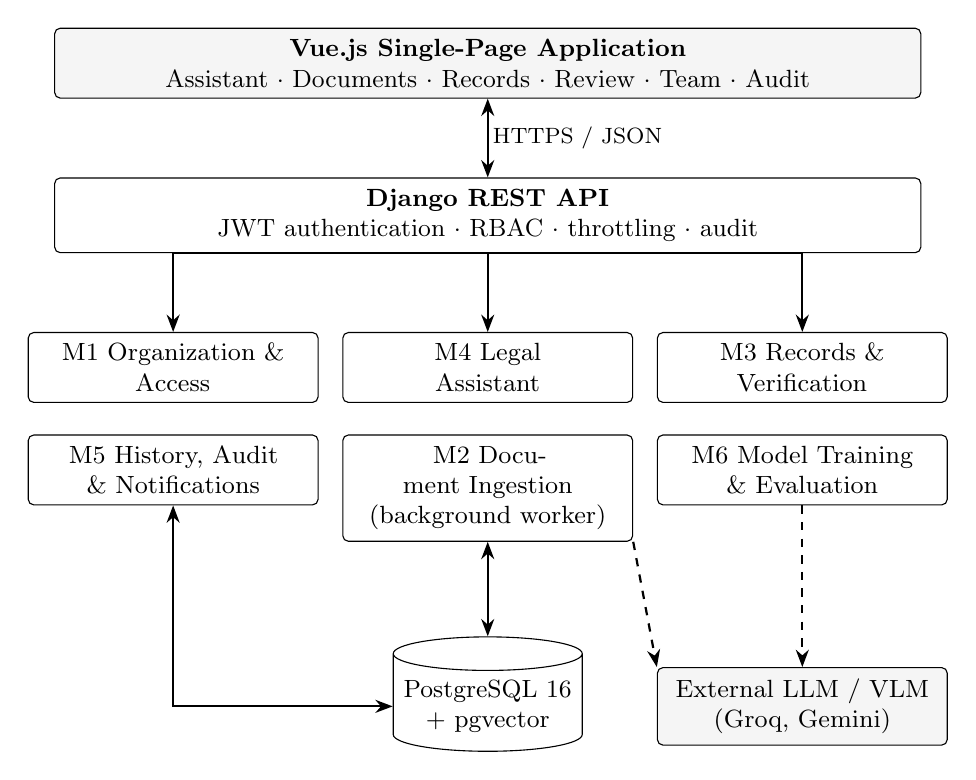
\begin{tikzpicture}[node distance=6mm and 6mm]
\node[box,minimum width=11cm,fill=gray!8] (ui) {\textbf{Vue.js Single-Page Application}\\ Assistant $\cdot$ Documents $\cdot$ Records $\cdot$ Review $\cdot$ Team $\cdot$ Audit};
\node[box,below=10mm of ui,minimum width=11cm] (api) {\textbf{Django REST API}\\ JWT authentication $\cdot$ RBAC $\cdot$ throttling $\cdot$ audit};
\node[box,below=10mm of api,text width=34mm] (m4) {M4 Legal\\ Assistant};
\node[box,left=3mm of m4,text width=34mm] (m1) {M1 Organization \&\\ Access};
\node[box,right=3mm of m4,text width=34mm] (m3) {M3 Records \&\\ Verification};
\node[box,below=4mm of m1,text width=34mm] (m5) {M5 History, Audit\\ \& Notifications};
\node[box,below=4mm of m4,text width=34mm] (m2) {M2 Document Ingestion\\ (background worker)};
\node[box,below=4mm of m3,text width=34mm] (m6) {M6 Model Training\\ \& Evaluation};
\node[db,below=12mm of m2] (db) {PostgreSQL 16\\ + pgvector};
\node[box,fill=gray!8,text width=34mm] (llm) at (m6 |- db) {External LLM / VLM\\ (Groq, Gemini)};
\draw[<->,thick] (ui) -- node[lbl,right]{HTTPS / JSON} (api);
\draw[->,thick] (api) -- (m4.north);
\draw[->,thick] (api.south) -| (m1.north);
\draw[->,thick] (api.south) -| (m3.north);
\draw[<->,thick] (m2) -- (db);
\draw[<->,thick] (m5.south) |- (db.west);
\draw[->,dashed,thick] (m2.south east) -- (llm.north west);
\draw[->,dashed,thick] (m6) -- (llm);
\end{tikzpicture}
\caption{High-Level System Architecture of \sysname{}}\label{fig:highlevel}
\end{figure}

\subsection{Module 1: Organization and Access Management}
Registers an organization and its first administrator, authenticates users with JSON Web Tokens, and
lets administrators add members, assign roles and departments. It defines the access model used by
every other module: a user sees all organization-wide documents, the documents of their department,
documents they uploaded and documents shared with them by name; Admins and Auditors see all documents
of the organization.

\subsection{Module 2: Document Ingestion and Processing}
Validates uploads, stores each file as a numbered version, and queues it for the background worker.
The worker extracts text page by page, chooses between the digital text layer, Tesseract OCR and the
vision-language model for each page, classifies the document, chunks it by section, computes
embeddings, labels contract clauses with the fine-tuned classifier, and extracts record fields.
Users can upload new versions and compare any two versions line by line.

\subsection{Module 3: Records Register and Verification}
Presents all records of the organization as one register (title, type, parties, dates, status) that
can be filtered and sorted. Each field shows its evidence quote and page. Fields marked
\emph{Needs review} appear in a review queue where Managers and Admins verify or correct them; every
change is stored in the field's edit history.

\subsection{Module 4: Legal Assistant}
Accepts a question, optionally limited to selected documents. A router (an LLM with a keyword fallback)
classifies the question as LOOKUP, KNOWLEDGE or SEARCH and extracts filters such as document type,
party, field and date range. Lookups are answered from the records table; knowledge questions are
answered by an LLM from hybrid-retrieved passages with numbered citations; searches return ranked
documents. Each conversation is saved.

\subsection{Module 5: History, Audit and Notifications}
Writes an append-only audit event for logins, uploads, views, downloads, searches, field edits, access
changes and membership changes. It also produces notifications: when a document is processed or fails,
when fields need review, and reminders 90, 30 and 7 days before (and on the day of) an expiry or a
notice deadline, sent only to people who can see the document.

\subsection{Module 6: Model Training and Evaluation}
Contains the scripts that fine-tune the clause classifier on LEDGAR, the TF-IDF and zero-shot LLM
baselines, and the evaluation suite that measures each AI component on CUAD, LEDGAR, a labelled
routing set and a handwriting set.

\section{Assumptions and Dependencies}
\begin{itemize}
\item Users have a modern web browser and network access to the server.
\item Uploaded documents are in English and reasonably legible.
\item An API key for at least one supported LLM provider (Groq, Gemini, OpenAI or a local Ollama server)
is configured; without it, upload, search, lookup and access control still work, while generated
answers and field extraction are disabled.
\item The server provides PostgreSQL 16 with pgvector and the Tesseract OCR engine.
\item The organization assigns roles responsibly; an administrator is trusted to manage members.
\end{itemize}

\section{Chapter Summary}
This chapter defined the problem of finding, trusting and protecting information in an organization's
legal documents, presented the proposed solution, its objectives and scope, and described the six
modules of the system. The next chapter analyzes the requirements in detail.

\chapter{Requirement Analysis}

\section{Introduction to Requirement Analysis}
This chapter specifies what \sysname{} must do (functional requirements) and how well it must do it
(non-functional requirements). The requirements were refined over several iterations: the first
version of the project was a general document chat tool, and the requirements below are the result of
re-scoping it into a legal records system for organizations.

\section{Requirement Elicitation Techniques}
\begin{itemize}
\item \textbf{Supervisor interviews.} The supervisor described the expected capabilities: uploading and
querying documents, holding all the records of an organization, looking up facts such as when an NDA
was signed, extracting records from handwritten documents, answering questions from a long law book,
role-based access with a shared document database, opening the source document for each answer, and
maintaining history.
\item \textbf{Review of the previous version.} Weaknesses of the first version (generic scope, no roles,
no structured data, no history, fixed-size chunks) were listed and turned into requirements.
\item \textbf{Document analysis.} Sample NDAs, leases, service agreements, employment letters, affidavits
and the Contract Act 1872 were studied to decide which fields to extract and how legal documents are
structured (parts, chapters, sections, numbered clauses).
\item \textbf{Analysis of existing systems.} The tools in Section~1.3 were studied to identify gaps.
\item \textbf{Prototyping.} Interface prototypes were reviewed and refined iteratively.
\end{itemize}

\section{User Classes and Characteristics}
\begin{table}[H]\centering
\caption{User Classes and Characteristics}\label{tab:userclasses}
\begin{tabularx}{\textwidth}{|p{2.6cm}|X|X|}\hline
\textbf{User Class} & \textbf{Characteristics} & \textbf{Permissions} \\ \hline
Admin & Owner or IT/legal lead of the organization; registers the organization. &
Everything: manage members, roles and departments; see all documents; verify fields; view audit log. \\ \hline
Manager & Department head or legal officer; responsible for the accuracy of records. &
Upload; edit documents of their department; verify and correct extracted fields. \\ \hline
Employee & Regular staff member with basic computer skills. &
Upload; ask questions and open documents they are allowed to see; edit their own uploads. \\ \hline
Auditor & Internal or external auditor; must not change anything. &
Read-only access to all documents of the organization and to the audit log; cannot upload. \\ \hline
Background Worker (system) & Process that runs the processing pipeline. &
Reads queued versions and writes pages, chunks, fields and notifications. \\ \hline
\end{tabularx}
\end{table}

\section{System Overview}
Users interact with \sysname{} through a browser. After signing in, they land on the Assistant, where
they ask questions about the organization's documents. From the Documents screen they upload files,
open documents, see their versions, extracted facts, clauses and activity, and change who can see
them. The Records screen lists every record with its key fields; the Review screen lists values waiting
for human confirmation. Administrators manage members and departments, and Admins and Auditors can read
the audit log. All processing happens in the background and users are notified when it finishes.

\section{Use Case Model}
\subsection{Use Case Diagram}
Figure~\ref{fig:usecase} shows the actors and the main use cases. Managers and Admins inherit all
Employee use cases; Auditors have read-only use cases and the audit log.

\begin{figure}[H]\centering
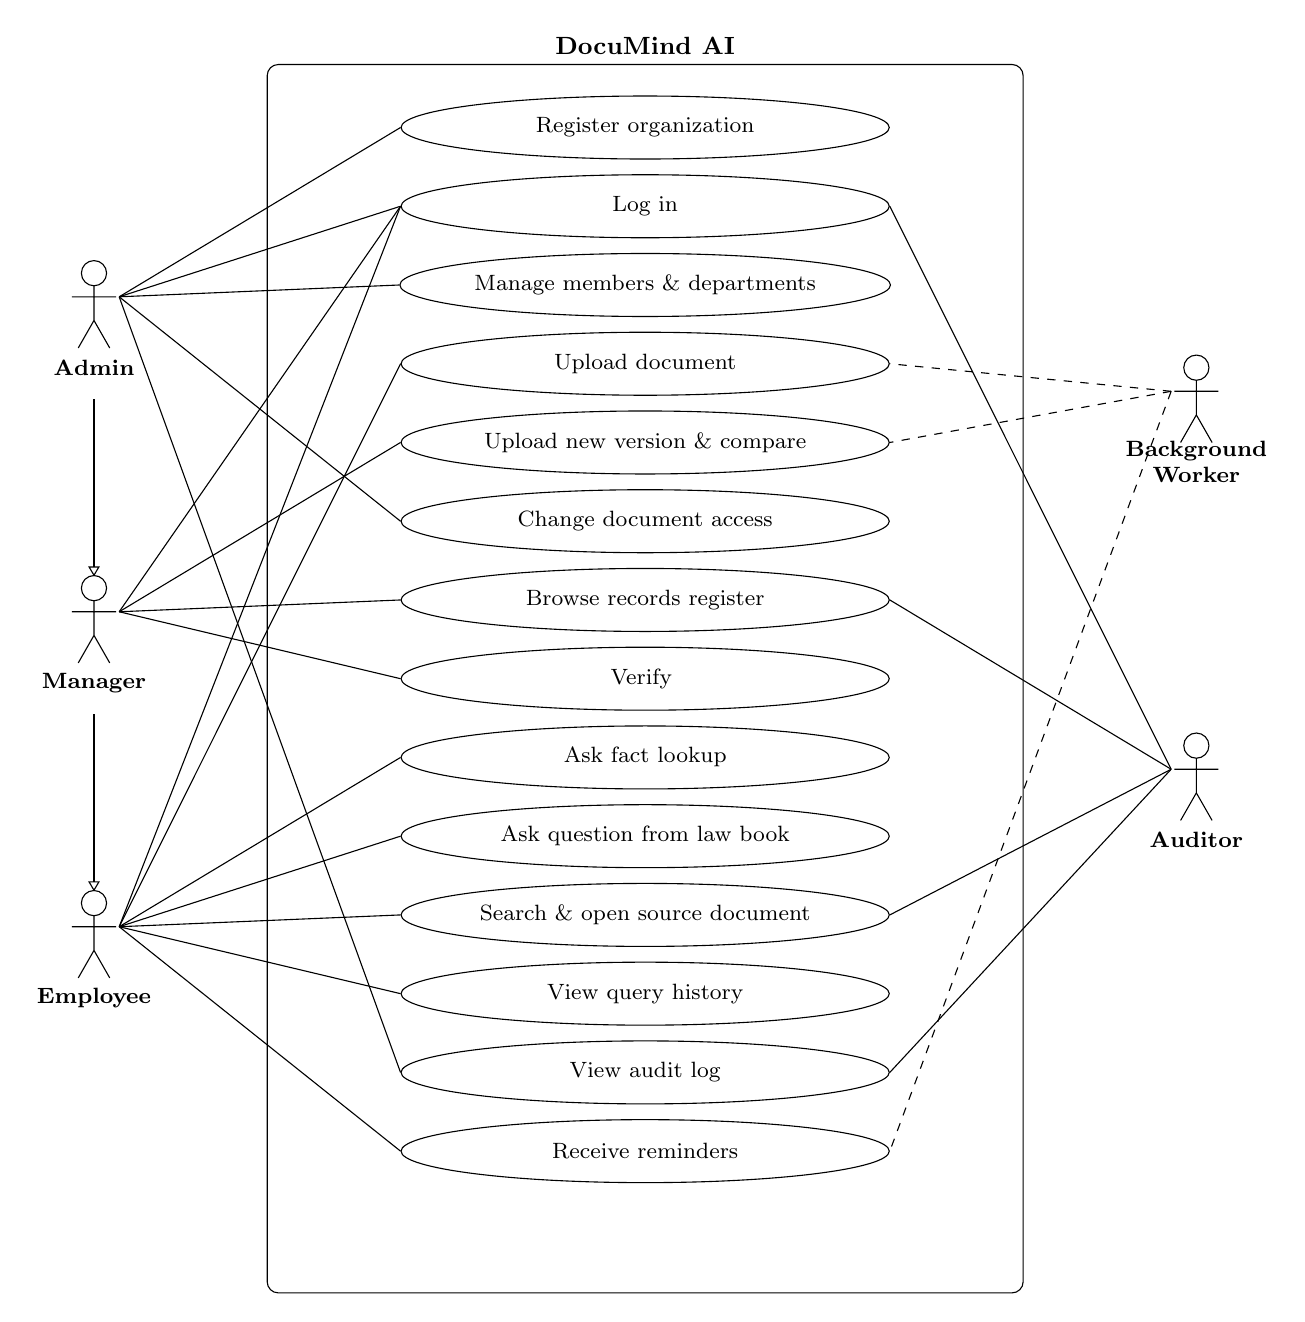
\begin{tikzpicture}[x=1cm,y=1cm]
\node[draw,rounded corners=4pt,minimum width=9.6cm,minimum height=15.6cm,label={[font=\small\bfseries]north:\sysname{}}] (sys) at (0,0) {};
\foreach \n/\y/\t in {
  u11/7.0/Register organization, u12/6.0/Log in, u13/5.0/Manage members \& departments,
  u21/4.0/Upload document, u22/3.0/Upload new version \& compare, u23/2.0/Change document access,
  u31/1.0/Browse records register, u32/0.0/Verify / correct field,
  u41/-1.0/Ask fact lookup, u42/-2.0/Ask question from law book, u43/-3.0/Search \& open source document,
  u44/-4.0/View query history, u51/-5.0/View audit log, u52/-6.0/Receive reminders}
  {\node[usecase,minimum width=62mm] (\n) at (0,\y) {\t};}
\actor{adm}{(-7,4.6)}{Admin}
\actor{mgr}{(-7,0.6)}{Manager}
\actor{emp}{(-7,-3.4)}{Employee}
\actor{aud}{(7,-1.4)}{Auditor}
\actor{wrk}{(7,3.4)}{Background\\Worker}
\foreach \u in {u11,u12,u13,u23,u51} \draw ([shift={(0.32,0.15)}]adm) -- (\u.west);
\foreach \u in {u12,u22,u31,u32} \draw ([shift={(0.32,0.15)}]mgr) -- (\u.west);
\foreach \u in {u12,u21,u41,u42,u43,u44,u52} \draw ([shift={(0.32,0.15)}]emp) -- (\u.west);
\foreach \u in {u12,u31,u43,u51} \draw ([shift={(-0.32,0.15)}]aud) -- (\u.east);
\foreach \u in {u21,u22,u52} \draw[dashed] ([shift={(-0.32,0.15)}]wrk) -- (\u.east);
\draw[-{Triangle[open]}] (-7,0.1) ++(0,-0.55) -- (-7,-2.7);
\draw[-{Triangle[open]}] (-7,4.1) ++(0,-0.55) -- (-7,1.3);
\end{tikzpicture}
\caption{Use Case Diagram of the Proposed System}\label{fig:usecase}
\end{figure}

\subsection{Use Case Descriptions}

\subsubsection{Module 1: Organization and Access Management}
\begin{spec}{UC-1.1: Register Organization}{tab:uc11}
\row{Use Case ID}{UC-1.1}
\row{Use Case Name}{Register Organization}
\row{Actors}{Admin (new)}
\row{Description}{A person creates a new organization in \sysname{} and becomes its first administrator.}
\row{Trigger}{The user selects ``Get started'' on the landing page.}
\row{Preconditions}{The username and e-mail are not already registered.}
\row{Postconditions}{An Organization, a User and an Admin Membership are created; the user is signed in.}
\row{Normal Flow}{\begin{steps}
\item User enters organization name, full name, username, e-mail and password.
\item System validates the fields and password strength.
\item System creates the organization, the user and the Admin membership in one transaction.
\item System returns tokens and opens the Assistant.
\end{steps}}
\row{Alternative Flow}{If validation fails or the username exists, the system shows the error next to the field and nothing is created.}
\end{spec}

\begin{spec}{UC-1.2: Log In}{tab:uc12}
\row{Use Case ID}{UC-1.2}
\row{Use Case Name}{Log In}
\row{Actors}{Admin, Manager, Employee, Auditor}
\row{Description}{A registered member signs in to access the organization's documents.}
\row{Trigger}{The user opens the Login page and submits credentials.}
\row{Preconditions}{The user has an active account and an organization membership.}
\row{Postconditions}{An access token (8 hours) and refresh token (7 days) are issued; a LOGIN audit event is written.}
\row{Normal Flow}{\begin{steps}
\item User enters username and password.
\item System verifies the password hash.
\item System issues JWT tokens and records the login.
\item System opens the Assistant with the user's name, role and organization.
\end{steps}}
\row{Alternative Flow}{Wrong credentials: the system shows ``Invalid username or password'' and issues no token.}
\end{spec}

\begin{spec}{UC-1.3: Manage Members and Departments}{tab:uc13}
\row{Use Case ID}{UC-1.3}
\row{Use Case Name}{Manage Members and Departments}
\row{Actors}{Admin}
\row{Description}{The administrator adds members, assigns roles and departments, and creates departments.}
\row{Trigger}{Admin opens the Team screen.}
\row{Preconditions}{The user is an Admin.}
\row{Postconditions}{Membership changes are saved and recorded as MEMBER\_ADD / MEMBER\_UPDATE / DEPARTMENT\_CHANGE audit events.}
\row{Normal Flow}{\begin{steps}
\item Admin selects ``Add member'' and enters name, username, e-mail, temporary password, role and department.
\item System creates the user and membership in the admin's organization.
\item Admin may later change a member's role or department.
\end{steps}}
\row{Alternative Flow}{A non-admin calling the API receives HTTP 403. Duplicate usernames are rejected.}
\end{spec}

\subsubsection{Module 2: Document Ingestion and Processing}
\begin{spec}{UC-2.1: Upload Document}{tab:uc21}
\row{Use Case ID}{UC-2.1}
\row{Use Case Name}{Upload Document}
\row{Actors}{Employee, Manager, Admin; Background Worker}
\row{Description}{A user adds a document to the shared repository; the worker processes it.}
\row{Trigger}{User selects ``Upload'' and chooses one or more files.}
\row{Preconditions}{User's role can upload. File is PDF, DOCX, PNG or JPG and at most 25\,MB.}
\row{Postconditions}{Document and version 1 exist; a processing job is queued; when finished the version is READY with pages, chunks and (for records) fields; the uploader is notified.}
\row{Normal Flow}{\begin{steps}
\item User chooses files, optionally a title, department, access level, document kind and the ``handwritten'' flag.
\item System validates type and size, stores the file and computes its SHA-256 hash.
\item System creates the document, version 1 and a queued job, and writes an UPLOAD audit event.
\item Worker extracts text, classifies, chunks, embeds, labels clauses and extracts fields.
\item Status changes to Ready and a notification is sent.
\end{steps}}
\row{Alternative Flow}{Invalid type or size: rejected with a message. Processing error: the job is retried up to 3 times, then the version is marked FAILED and the uploader is notified.}
\end{spec}

\begin{spec}{UC-2.2: Upload New Version and Compare}{tab:uc22}
\row{Use Case ID}{UC-2.2}
\row{Use Case Name}{Upload New Version and Compare}
\row{Actors}{Manager, Admin, uploader of the document}
\row{Description}{A signed or amended copy replaces the current one while older versions are kept.}
\row{Trigger}{User selects ``New version'' on a document.}
\row{Preconditions}{User may edit the document.}
\row{Postconditions}{Version $n+1$ is stored and processed; when ready it becomes the current version; earlier versions remain viewable.}
\row{Normal Flow}{\begin{steps}
\item User uploads the new file with a change note.
\item System stores it as the next version and queues processing.
\item User selects two versions and ``Compare''.
\item System shows added and removed lines and the field values that changed.
\end{steps}}
\row{Alternative Flow}{If the user may not edit the document, HTTP 403 is returned.}
\end{spec}

\begin{spec}{UC-2.3: Change Document Access}{tab:uc23}
\row{Use Case ID}{UC-2.3}
\row{Use Case Name}{Change Document Access}
\row{Actors}{Admin, Manager (own department), uploader}
\row{Description}{The user sets who may see a document: everyone, one department, or named people.}
\row{Trigger}{User opens the document's settings.}
\row{Preconditions}{User may edit the document.}
\row{Postconditions}{Access level and shared users are saved; an ACCESS\_CHANGE audit event is written; search results change immediately.}
\row{Normal Flow}{\begin{steps}
\item User chooses Organization, Department or Restricted, and selects people for Restricted.
\item System saves the setting and logs it.
\end{steps}}
\row{Alternative Flow}{Unauthorized users do not see the settings button; the API returns 403.}
\end{spec}

\subsubsection{Module 3: Records Register and Verification}
\begin{spec}{UC-3.1: Browse Records Register}{tab:uc31}
\row{Use Case ID}{UC-3.1}
\row{Use Case Name}{Browse Records Register}
\row{Actors}{All roles}
\row{Description}{The user sees every visible record with its key fields in one table.}
\row{Trigger}{User opens the Records screen.}
\row{Preconditions}{User is signed in.}
\row{Postconditions}{None (read-only).}
\row{Normal Flow}{\begin{steps}
\item System lists visible records with type, parties, signing, effective and expiry dates and status.
\item User filters by text or type and sorts by a column.
\item User opens a record to see each field with its evidence quote.
\end{steps}}
\row{Alternative Flow}{If no records exist, an empty state explains how to upload.}
\end{spec}

\begin{spec}{UC-3.2: Verify or Correct Field}{tab:uc32}
\row{Use Case ID}{UC-3.2}
\row{Use Case Name}{Verify or Correct Extracted Field}
\row{Actors}{Manager, Admin}
\row{Description}{A reviewer confirms or corrects a value the system was not sure about.}
\row{Trigger}{Reviewer opens the Review queue or a field on a document.}
\row{Preconditions}{User can verify; the field belongs to a document they can see.}
\row{Postconditions}{Field status becomes VERIFIED or CORRECTED; a FieldEdit history row and an audit event are written.}
\row{Normal Flow}{\begin{steps}
\item System shows the value, its confidence and the quote, and opens the page with the quote highlighted.
\item Reviewer selects ``Verify'' or enters the correct value and a reason.
\item System saves the change and removes the field from the queue.
\end{steps}}
\row{Alternative Flow}{Employees and Auditors receive HTTP 403 when trying to verify.}
\end{spec}

\subsubsection{Module 4: Legal Assistant}
\begin{spec}{UC-4.1: Ask a Fact Lookup}{tab:uc41}
\row{Use Case ID}{UC-4.1}
\row{Use Case Name}{Ask a Fact Lookup}
\row{Actors}{All roles}
\row{Description}{The user asks for a stored fact, e.g.\ ``When was the NDA with Acme signed?''.}
\row{Trigger}{User submits a question in the Assistant.}
\row{Preconditions}{User is signed in; at least one processed record is visible.}
\row{Postconditions}{Answer, sources and plan are saved to the conversation; a SEARCH audit event is written.}
\row{Normal Flow}{\begin{steps}
\item Router classifies the question as LOOKUP with filters (type NDA, party Acme, field signed\_date).
\item System queries the records table, limited to visible documents.
\item System answers with the value, the document and the page, and lists the evidence as a source.
\item User clicks the source; the document opens at that page with the quote highlighted.
\end{steps}}
\row{Alternative Flow}{No matching record: the system falls back to passage search and says when nothing is found.}
\end{spec}

\begin{spec}{UC-4.2: Ask a Question from a Law Book}{tab:uc42}
\row{Use Case ID}{UC-4.2}
\row{Use Case Name}{Ask a Question from Reference Material}
\row{Actors}{All roles}
\row{Description}{The user asks for an explanation, e.g.\ ``Is an agreement without consideration valid under the Contract Act?''.}
\row{Trigger}{User submits a question.}
\row{Preconditions}{The reference document has been processed and is visible to the user.}
\row{Postconditions}{Answer with citations is saved to the conversation.}
\row{Normal Flow}{\begin{steps}
\item Router classifies the question as KNOWLEDGE.
\item Hybrid retrieval returns the 8 best passages from visible documents.
\item LLM writes an answer using only those passages, with [n] citations.
\item System shows the answer and the cited passages with section and page.
\end{steps}}
\row{Alternative Flow}{If the passages do not contain the answer, the system says so. If the LLM is unavailable, the most relevant passages are shown without a written answer.}
\end{spec}

\begin{spec}{UC-4.3: Search and Open Source Document}{tab:uc43}
\row{Use Case ID}{UC-4.3}
\row{Use Case Name}{Search and Open Source Document}
\row{Actors}{All roles}
\row{Description}{The user asks to find documents, e.g.\ ``Find the lease for the Lahore office''.}
\row{Trigger}{User submits a search-style question or uses the command palette.}
\row{Preconditions}{User is signed in.}
\row{Postconditions}{Matching documents are listed; opening one writes a VIEW audit event.}
\row{Normal Flow}{\begin{steps}
\item Router classifies the question as SEARCH.
\item System ranks visible documents by their best-matching passages and clause labels.
\item User opens a result in the document viewer.
\end{steps}}
\row{Alternative Flow}{No results: the system suggests rephrasing.}
\end{spec}

\begin{spec}{UC-4.4: View Query History}{tab:uc44}
\row{Use Case ID}{UC-4.4}
\row{Use Case Name}{View Query History}
\row{Actors}{All roles}
\row{Description}{The user reopens an earlier conversation with its answers and sources.}
\row{Trigger}{User selects a conversation from the history list.}
\row{Preconditions}{The conversation belongs to the user.}
\row{Postconditions}{None.}
\row{Normal Flow}{\begin{steps}
\item System lists the user's conversations, newest first.
\item User opens one; all questions, answers, sources and timings are shown.
\end{steps}}
\row{Alternative Flow}{Another user's conversation id returns HTTP 404.}
\end{spec}

\subsubsection{Module 5: History, Audit and Notifications}
\begin{spec}{UC-5.1: View Audit Log}{tab:uc51}
\row{Use Case ID}{UC-5.1}
\row{Use Case Name}{View Audit Log}
\row{Actors}{Admin, Auditor}
\row{Description}{The user reviews who did what and when in the organization.}
\row{Trigger}{User opens the Audit screen.}
\row{Preconditions}{User is an Admin or Auditor.}
\row{Postconditions}{None (events cannot be edited or deleted).}
\row{Normal Flow}{\begin{steps}
\item System lists events with time, person, action, target and details.
\item User filters by action, person or text.
\end{steps}}
\row{Alternative Flow}{Other roles receive HTTP 403 and do not see the menu item.}
\end{spec}

\begin{spec}{UC-5.2: Receive Reminders}{tab:uc52}
\row{Use Case ID}{UC-5.2}
\row{Use Case Name}{Receive Expiry and Notice Reminders}
\row{Actors}{Background Worker; uploader, department managers and admins}
\row{Description}{The system warns responsible people before an agreement expires or its notice deadline passes.}
\row{Trigger}{Hourly reminder check in the worker.}
\row{Preconditions}{A record has an expiry date (and optionally a notice period).}
\row{Postconditions}{One notification per person per reminder window; optional e-mail.}
\row{Normal Flow}{\begin{steps}
\item Worker finds expiry dates and notice deadlines (expiry minus notice period) 90, 30, 7 or 0 days ahead.
\item It selects people who can see the document: the uploader, managers of its department and admins.
\item It creates a notification for each, skipping ones already sent.
\end{steps}}
\row{Alternative Flow}{People who cannot see the document are never notified.}
\end{spec}

\subsection{Event-Response Table}
\begin{table}[H]\centering
\caption{Event-Response Table}\label{tab:events}
\begin{tabularx}{\textwidth}{|p{4.6cm}|X|}\hline
\textbf{Event} & \textbf{System Response} \\ \hline
User submits a valid upload & Store file as a new version, queue a job, log UPLOAD, show ``Queued'' status. \\ \hline
Worker finishes a job & Mark version READY, make it current, notify the uploader; notify reviewers if fields need review. \\ \hline
Processing fails three times & Mark version FAILED with the error, notify the uploader. \\ \hline
User asks a question & Route, retrieve from visible documents only, answer with sources, save to history, log SEARCH. \\ \hline
User opens or downloads a document & Check access, stream the file, log VIEW / DOWNLOAD. \\ \hline
Reviewer verifies or corrects a field & Update status/value, store FieldEdit, log FIELD\_VERIFY / FIELD\_EDIT. \\ \hline
Admin changes a role or department & Update membership, log MEMBER\_UPDATE; access changes apply to the next request. \\ \hline
Hourly reminder check & Create due expiry / notice reminders without duplicates. \\ \hline
LLM provider rate-limits a call & Retry within a deadline, then switch to the fallback provider; if both fail, show passages without a written answer. \\ \hline
\end{tabularx}
\end{table}

\section{Functional Requirements}
Each requirement below has an identifier used in the traceability matrix (Table~\ref{tab:rtm}).

\subsection{Module 1: Organization and Access Management}
\subsubsection{FR-1.1 Organization Registration and Authentication}
\begin{spec}{Functional Requirement -- Registration and Authentication}{tab:fr11}
\row{Identifier}{FR-1.1}
\row{Title}{Organization registration and authentication}
\row{Requirement}{The system shall let a person register an organization and become its Admin, and shall authenticate members with username and password, issuing JWT access (8 h) and refresh (7 days) tokens.}
\row{Source}{Supervisor; previous version}
\row{Rationale}{Every document belongs to an organization; identity is required for access control and auditing.}
\row{Dependencies}{None}
\row{Priority}{High}
\end{spec}

\subsubsection{FR-1.2 Members, Departments and Roles}
\begin{spec}{Functional Requirement -- Members, Departments and Roles}{tab:fr12}
\row{Identifier}{FR-1.2}
\row{Title}{Member and department management}
\row{Requirement}{An Admin shall be able to add members, create departments, and assign each member one role (Admin, Manager, Employee, Auditor) and optionally one department.}
\row{Source}{Supervisor (RBAC, shared database)}
\row{Dependencies}{FR-1.1}
\row{Priority}{High}
\end{spec}

\subsubsection{FR-1.3 Document Access Control}
\begin{spec}{Functional Requirement -- Document Access Control}{tab:fr13}
\row{Identifier}{FR-1.3}
\row{Title}{Access control before retrieval}
\row{Requirement}{Each document shall have an access level (Organization, Department, Restricted to named people). A member shall see a document only if it is organization-wide, belongs to their department, was uploaded by them or was shared with them; Admins and Auditors see all. This rule shall be applied before every list, search, retrieval, file download and answer.}
\row{Source}{Supervisor (RBAC)}
\row{Dependencies}{FR-1.2}
\row{Priority}{High}
\end{spec}

\subsection{Module 2: Document Ingestion and Processing}
\subsubsection{FR-2.1 Upload and Validation}
\begin{spec}{Functional Requirement -- Upload and Validation}{tab:fr21}
\row{Identifier}{FR-2.1}
\row{Title}{Document upload}
\row{Requirement}{The system shall accept PDF, DOCX, PNG, JPG and JPEG files up to 25\,MB, store each as a numbered version with its SHA-256 hash, and process it in the background. Auditors shall not be able to upload.}
\row{Dependencies}{FR-1.3}
\row{Priority}{High}
\end{spec}

\subsubsection{FR-2.2 Text Extraction, OCR and Handwriting}
\begin{spec}{Functional Requirement -- Text Extraction, OCR and Handwriting}{tab:fr22}
\row{Identifier}{FR-2.2}
\row{Title}{Reading every page}
\row{Requirement}{For each page the system shall use the digital text layer when present; otherwise run Tesseract OCR; and if the uploader marked the document handwritten, or Tesseract's mean confidence is below 70 or it finds almost no words, transcribe the page with a vision-language model. The source of each page (Digital, OCR, Handwriting) shall be stored.}
\row{Source}{Supervisor (handwritten records)}
\row{Dependencies}{FR-2.1}
\row{Priority}{High}
\end{spec}

\subsubsection{FR-2.3 Classification}
\begin{spec}{Functional Requirement -- Record / Reference Classification}{tab:fr23}
\row{Identifier}{FR-2.3}
\row{Title}{Document classification}
\row{Requirement}{The system shall classify every document as RECORD or REFERENCE, assign a document type and a one-sentence summary. A user may set the kind manually, after which it is not changed automatically.}
\row{Dependencies}{FR-2.2}
\row{Priority}{Medium}
\end{spec}

\subsubsection{FR-2.4 Structure-aware Chunking and Indexing}
\begin{spec}{Functional Requirement -- Chunking and Indexing}{tab:fr24}
\row{Identifier}{FR-2.4}
\row{Title}{Chunking and indexing}
\row{Requirement}{The system shall split text at legal headings (Part, Chapter, Article, Section, numbered clauses, capitalized titles) into chunks of at most 1,500 characters that keep their section path and page range, and index each chunk with a 384-dimensional embedding and a weighted full-text vector.}
\row{Dependencies}{FR-2.2}
\row{Priority}{High}
\end{spec}

\subsubsection{FR-2.5 Versions and Comparison}
\begin{spec}{Functional Requirement -- Versions and Comparison}{tab:fr25}
\row{Identifier}{FR-2.5}
\row{Title}{Document versions}
\row{Requirement}{Users who may edit a document shall be able to upload a new version with a change note. Older versions shall never be deleted, and any two versions shall be comparable (text differences and changed fields).}
\row{Source}{Supervisor (history)}
\row{Dependencies}{FR-2.1}
\row{Priority}{High}
\end{spec}

\subsubsection{FR-2.6 Clause Labelling}
\begin{spec}{Functional Requirement -- Clause Labelling}{tab:fr26}
\row{Identifier}{FR-2.6}
\row{Title}{Clause labelling with a fine-tuned model}
\row{Requirement}{Chunks of RECORD documents shall be labelled with one of 100 clause types by the fine-tuned classifier when its confidence is at least 0.5, and labels shall be shown on the document and used to boost search.}
\row{Source}{Supervisor (fine-tuning)}
\row{Dependencies}{FR-2.4}
\row{Priority}{Medium}
\end{spec}

\subsection{Module 3: Records Register and Verification}
\subsubsection{FR-3.1 Field Extraction with Evidence}
\begin{spec}{Functional Requirement -- Field Extraction with Evidence}{tab:fr31}
\row{Identifier}{FR-3.1}
\row{Title}{Record field extraction}
\row{Requirement}{For RECORD documents the system shall extract eleven fields (parties, effective date, signing date, expiry date, term, auto-renewal, notice period, governing law, contract value, reference number, signatories), each with a page number, a verbatim quote and a confidence. Dates shall be normalized to ISO format and amounts to numbers. The quote shall be checked against the page text (grounding).}
\row{Source}{Supervisor (``when was the NDA signed'')}
\row{Dependencies}{FR-2.2, FR-2.3}
\row{Priority}{High}
\end{spec}

\subsubsection{FR-3.2 Review Queue}
\begin{spec}{Functional Requirement -- Review Queue}{tab:fr32}
\row{Identifier}{FR-3.2}
\row{Title}{Human review of uncertain values}
\row{Requirement}{A field shall be marked NEEDS\_REVIEW when its confidence is below 0.75, its quote is not found on the page, or it comes from an OCR or handwritten page. Managers and Admins shall be able to verify or correct such fields.}
\row{Dependencies}{FR-3.1}
\row{Priority}{High}
\end{spec}

\subsubsection{FR-3.3 Field Edit History and Records Register}
\begin{spec}{Functional Requirement -- Field History and Register}{tab:fr33}
\row{Identifier}{FR-3.3}
\row{Title}{Field edit history and records register}
\row{Requirement}{Every verification or correction shall be stored with old and new value, old and new status, reason, person and time. The system shall provide a register of all visible records with their key fields, filterable and sortable.}
\row{Source}{Supervisor (history, hold all records)}
\row{Dependencies}{FR-3.2}
\row{Priority}{High}
\end{spec}

\subsection{Module 4: Legal Assistant}
\subsubsection{FR-4.1 Query Routing}
\begin{spec}{Functional Requirement -- Query Routing}{tab:fr41}
\row{Identifier}{FR-4.1}
\row{Title}{Query routing}
\row{Requirement}{The system shall classify each question as LOOKUP, KNOWLEDGE or SEARCH and extract document type, party, field and date range, using an LLM plan in JSON with a keyword-rule fallback. The LLM shall never write SQL.}
\row{Dependencies}{FR-3.1}
\row{Priority}{High}
\end{spec}

\subsubsection{FR-4.2 Lookup, Knowledge and Search Answers}
\begin{spec}{Functional Requirement -- Answer Engines}{tab:fr42}
\row{Identifier}{FR-4.2}
\row{Title}{Answering questions}
\row{Requirement}{LOOKUP questions shall be answered from the records table; KNOWLEDGE questions from the top 8 hybrid-retrieved passages with numbered citations; SEARCH questions with a ranked list of documents. A question may be limited to selected documents. If the sources do not contain the answer the system shall say so.}
\row{Source}{Supervisor (law book, fact lookup)}
\row{Dependencies}{FR-1.3, FR-2.4, FR-4.1}
\row{Priority}{High}
\end{spec}

\subsubsection{FR-4.3 Source Document Viewing}
\begin{spec}{Functional Requirement -- Source Viewing}{tab:fr43}
\row{Identifier}{FR-4.3}
\row{Title}{Open the source}
\row{Requirement}{Every source in an answer shall open the document at the cited page with the quoted text highlighted.}
\row{Source}{Supervisor (``the query pulls up the document'')}
\row{Dependencies}{FR-4.2}
\row{Priority}{High}
\end{spec}

\subsubsection{FR-4.4 Query History}
\begin{spec}{Functional Requirement -- Query History}{tab:fr44}
\row{Identifier}{FR-4.4}
\row{Title}{Conversation history}
\row{Requirement}{Each question shall be stored with its route, filters, scope, answer, sources and response time in a conversation that only its owner can open.}
\row{Source}{Supervisor (history)}
\row{Priority}{Medium}
\end{spec}

\subsection{Module 5: History, Audit and Notifications}
\subsubsection{FR-5.1 Audit Log}
\begin{spec}{Functional Requirement -- Audit Log}{tab:fr51}
\row{Identifier}{FR-5.1}
\row{Title}{Append-only audit log}
\row{Requirement}{The system shall record logins, uploads, new versions, views, downloads, searches, field edits and verifications, document updates, access changes, archiving, reprocessing and membership changes, with person, target, details, IP address and time. Events shall not be editable or deletable, and only Admins and Auditors may read them.}
\row{Source}{Supervisor (history)}
\row{Priority}{High}
\end{spec}

\subsubsection{FR-5.2 Notifications and Reminders}
\begin{spec}{Functional Requirement -- Notifications and Reminders}{tab:fr52}
\row{Identifier}{FR-5.2}
\row{Title}{Notifications and reminders}
\row{Requirement}{The system shall notify the uploader when processing finishes or fails, reviewers when fields need review, and responsible people 90, 30 and 7 days before and on the day of an expiry date or notice deadline, without duplicates and only to people who can see the document.}
\row{Priority}{Medium}
\end{spec}

\section{Non-Functional Requirements}
\subsection{Performance Requirements}
\begin{itemize}
\item \textbf{PER-1:} Lookup answers shall be returned within 3 seconds.
\item \textbf{PER-2:} Knowledge answers shall be returned within 35 seconds in the worst case; every LLM
call has a deadline after which the fallback provider or a passages-only answer is used.
\item \textbf{PER-3:} Uploading shall return immediately; processing runs in the background.
\item \textbf{PER-4:} Vector search shall use an HNSW index so that response time does not grow linearly with
the number of chunks.
\end{itemize}
\subsection{Security Requirements}
\begin{itemize}
\item \textbf{SEC-1:} Passwords shall be stored as salted hashes (Django PBKDF2).
\item \textbf{SEC-2:} All API endpoints except registration and login shall require a valid JWT.
\item \textbf{SEC-3:} Access control shall be enforced on the server before any data is read; document ids
sent by the client shall be filtered through the same rule.
\item \textbf{SEC-4:} Files shall only be served through a permission-checked endpoint, never from a public
media URL.
\item \textbf{SEC-5:} The assistant shall be rate-limited (20 questions per minute per user) and the API
in general (600 requests per hour per user).
\item \textbf{SEC-6:} API keys and secrets shall be read from environment variables, never stored in code.
\end{itemize}
\subsection{Reliability Requirements}
\begin{itemize}
\item \textbf{REL-1:} Failed processing jobs shall be retried up to three times; jobs left running by a
crashed worker shall be recovered.
\item \textbf{REL-2:} If the LLM is unavailable, upload, search, lookup and access control shall keep working.
\item \textbf{REL-3:} Processing a new version shall not remove the current searchable version until the new
one is ready.
\end{itemize}
\subsection{Usability Requirements}
\begin{itemize}
\item \textbf{USE-1:} Every extracted value and every answer shall show its evidence.
\item \textbf{USE-2:} A new user shall be able to ask a first question within one minute of signing in.
\item \textbf{USE-3:} The interface shall support keyboard use (command palette with Ctrl/\,\textsuperscript{$\wedge$}K, ``/'' to focus
the question box) and visible focus states.
\end{itemize}
\subsection{Scalability Requirements}
\begin{itemize}
\item \textbf{SCA-1:} Several workers shall be able to run in parallel without taking the same job.
\item \textbf{SCA-2:} The backend shall be stateless so that more API containers can be added.
\end{itemize}
\subsection{Maintainability Requirements}
\begin{itemize}
\item \textbf{MAI-1:} The LLM provider shall be changeable through configuration only.
\item \textbf{MAI-2:} Core behavior shall be covered by automated tests run with \code{python manage.py test}.
\item \textbf{MAI-3:} Evaluation results shall be reproducible with the provided scripts.
\end{itemize}

\section{External Interface Requirements}
\subsection{User Interface Requirements}
A responsive web interface with a sidebar for navigation, a question box docked at the bottom of the
Assistant, an embedded PDF viewer, and clear status labels (Queued, Processing, Ready, Failed, Needs
review, Verified). Errors are shown as messages next to the field or as notifications.
\subsection{Hardware Interface Requirements}
The server needs at least 4\,GB RAM (embedding and clause models run on the CPU) and disk space for
uploaded files. No special client hardware is required; a scanner or phone camera is used to create
images of paper documents.
\subsection{Software Interface Requirements}
PostgreSQL 16 with pgvector 0.8, Tesseract OCR 5, Python 3.12+, and an OpenAI-compatible LLM endpoint
(Groq, Gemini, OpenAI or Ollama). Clients need a current version of Chrome, Edge, Firefox or Safari.
\subsection{Communication Interface Requirements}
The browser communicates with the server via REST over HTTPS with JSON bodies and Bearer tokens. The
server reaches LLM providers over HTTPS. Optional reminder e-mails use SMTP.

\section{Assumptions and Dependencies}
The requirements assume that documents are in English, that members are added by a trusted
administrator, and that at least one LLM provider is reachable for generated answers and field
extraction. Accuracy of handwriting recognition depends on the quality of the scan.

\section{Requirement Traceability Matrix}
\begin{table}[H]\centering
\caption{Requirement Traceability Matrix}\label{tab:rtm}
\small
\begin{tabularx}{\textwidth}{|p{1.3cm}|X|p{1.9cm}|p{3.4cm}|p{2.6cm}|}\hline
\textbf{FR} & \textbf{Requirement} & \textbf{Use Case} & \textbf{Implemented in} & \textbf{Test} \\ \hline
FR-1.1 & Registration \& authentication & UC-1.1, 1.2 & accounts/views.py & BB-01, BB-02 \\ \hline
FR-1.2 & Members, departments, roles & UC-1.3 & accounts/views.py & BB-03 \\ \hline
FR-1.3 & Access control before retrieval & UC-2.3, 4.x & documents/access.py & UT-04, UT-05, UT-06, IT-03 \\ \hline
FR-2.1 & Upload \& validation & UC-2.1 & documents/views.py & UT-08, UT-09, BB-04 \\ \hline
FR-2.2 & Extraction, OCR, handwriting & UC-2.1 & pipeline/\allowbreak{}extract.py, ai/ocr.py & IT-01, EV-5 \\ \hline
FR-2.3 & Classification & UC-2.1 & pipeline/\allowbreak{}understanding.py & IT-01 \\ \hline
FR-2.4 & Chunking \& indexing & UC-2.1 & pipeline/chunking.py & UT-03, EV-2 \\ \hline
FR-2.5 & Versions \& comparison & UC-2.2 & documents/views.py & UT-10, BB-05 \\ \hline
FR-2.6 & Clause labelling & UC-2.1 & ai/clauses.py, ml/ & EV-1 \\ \hline
FR-3.1 & Field extraction with evidence & UC-3.1 & pipeline/\allowbreak{}understanding.py & UT-01, UT-02, EV-3 \\ \hline
FR-3.2 & Review queue & UC-3.2 & documents/views.py & UT-12, BB-07 \\ \hline
FR-3.3 & Field history \& register & UC-3.1, 3.2 & documents/views.py & UT-11, BB-06 \\ \hline
FR-4.1 & Query routing & UC-4.1--4.3 & assistant/router.py & UT-14 -- UT-16, EV-4 \\ \hline
FR-4.2 & Answer engines & UC-4.1--4.3 & assistant/engine.py & UT-17, IT-02, IT-04, BB-08, BB-09 \\ \hline
FR-4.3 & Source viewing & UC-4.1, 4.3 & DocumentViewer.vue & BB-10 \\ \hline
FR-4.4 & Query history & UC-4.4 & assistant/views.py & UT-18, BB-11 \\ \hline
FR-5.1 & Audit log & UC-5.1 & audit/ & UT-13, BB-12 \\ \hline
FR-5.2 & Notifications \& reminders & UC-5.2 & notifications/ & UT-19 -- UT-23 \\ \hline
\end{tabularx}
\end{table}

\chapter{Software Design}

\section{Introduction to Software Design}
This chapter turns the requirements of Chapter~3 into a design. It describes the methodology and
process model, the architecture, the behavioral models (activity, sequence and state diagrams), the
static structure (class diagram), the data flows, and the database design with its data dictionary.

\section{Design Methodology and Software Process Model}
\subsection{Design Methodology}
An object-oriented design methodology was used. Domain concepts are modeled as classes (Django
models) with clear responsibilities, and behavior that crosses several classes is placed in service
modules: \code{documents/access.py} (access rules), \code{documents/pipeline/} (processing steps),
\code{assistant/router.py}, \code{assistant/retrieval.py} and \code{assistant/engine.py} (question
answering), \code{audit/service.py} and \code{notifications/service.py}. Every call to an AI model
goes through the \code{ai} package, which hides the provider behind one interface.

Two design principles guided the work:
\begin{enumerate}
\item \textbf{Permission before retrieval.} The function \code{visible\_documents(user)} is the only
way any module obtains documents. Search, lookups, file downloads and answers all start from its result,
so the language model can never receive text from a document the user may not open.
\item \textbf{Evidence for every fact.} Extracted values store their page and verbatim quote, answers
store their sources, and the interface always shows them. A value that cannot be proved is not trusted
automatically.
\end{enumerate}

\subsection{Software Process Model}
The project followed an iterative, incremental Agile process. Work was divided into short iterations,
each ending with a working, tested increment:
\begin{enumerate}
\item Domain re-scoping, data model, RBAC and the four history types.
\item Processing pipeline: extraction, OCR, handwriting, classification, chunking, embeddings.
\item Record field extraction with grounding, the review queue and the records register.
\item Query router, hybrid retrieval and the three answer engines with citations.
\item User interface redesign with the evidence-linked document viewer.
\item Clause classifier fine-tuning, the evaluation suite, reminders and deployment.
\end{enumerate}
This model suited the project because requirements from the supervisor were refined during
development and each increment could be demonstrated.

\section{System Overview}
Figure~\ref{fig:context} shows \sysname{} as a single process with its external entities. Members
(Admins, Managers, Employees and Auditors) provide documents, questions, verifications and
administrative data and receive answers, documents, review items and reminders. The system sends
prompts and page images to the LLM/VLM provider and optionally sends reminder e-mails.

\tikzfig[0.5]{context}{Context Diagram of \sysname{}}{fig:context}

\section{Architectural Design}
Figure~\ref{fig:architecture} shows the architecture. It is a layered client-server architecture with a
separate background worker.

\tikzfig[0.62]{architecture}{System Architecture Diagram of \sysname{}}{fig:architecture}

\begin{enumerate}
\item \textbf{Presentation tier (Vue.js 3 SPA).} Renders all screens, keeps the session token, and
calls the REST API. It contains no business rules; buttons a user may not use are hidden, but the server
enforces every rule again.
\item \textbf{Application tier (Django REST API).} Organized as five Django applications:
\code{accounts} (organizations, members, roles), \code{documents} (documents, versions, pages, chunks,
records, review), \code{assistant} (router, engines, retrieval, conversations), \code{audit} and
\code{notifications}. The \code{ai} package contains the LLM gateway (with deadline and provider
fallback), the embedding model, OCR and the clause classifier.
\item \textbf{Background worker.} A long-running \code{run\_worker} command claims queued jobs from a
database table using \code{SELECT \dots{} FOR UPDATE SKIP LOCKED}, runs the pipeline, retries failures
up to three times and runs the reminder check every hour. Using the database as the queue avoids an extra
message broker and works on Windows and Linux.
\item \textbf{Data tier.} PostgreSQL 16 holds all relational data. The pgvector extension stores chunk
embeddings with an HNSW index (cosine distance), and a weighted \code{tsvector} column with a GIN index
supports full-text search, so permission filters, vector search and keyword search run in the same
database. Uploaded files are stored on disk under organization- and document-specific paths and are
served only through a permission-checked endpoint.
\item \textbf{External services.} An OpenAI-compatible LLM endpoint (Groq by default, Gemini as
fallback) and a vision-language model for handwriting.
\end{enumerate}

\section{Design Models}
\subsection{Activity Diagrams}
\subsubsection{Module 2: Document Ingestion}
Figure~\ref{fig:act-ingest} shows how an uploaded file becomes searchable. Each page chooses its own
reading method, so a PDF that mixes typed pages with a handwritten signature page is handled correctly.

\tikzfig[0.82]{activity_ingestion}{Activity Diagram -- Document Ingestion}{fig:act-ingest}

\subsubsection{Module 4: Answering a Question}
Figure~\ref{fig:act-query} shows the three answer paths. All paths start from the user's visible
documents.

\tikzfig[0.8]{activity_query}{Activity Diagram -- Answering a Question}{fig:act-query}

\subsubsection{Module 3: Review and Verification}
\tikzfig[0.6]{activity_review}{Activity Diagram -- Review and Verification}{fig:act-review}

\subsubsection{Module 1: Organization and Member Management}
\tikzfig[0.7]{activity_users}{Activity Diagram -- Organization and Member Management}{fig:act-users}

\subsection{Class Diagram}
Figure~\ref{fig:class} shows the main classes, their key attributes and operations, and their
relationships. Filled diamonds mark composition: versions, pages, chunks and fields cannot exist without
their parent.

\tikzfig[0.8]{class_diagram}{Class Diagram of \sysname{}}{fig:class}

\subsection{Sequence Diagrams}
\subsubsection{Sequence Diagram -- User Login}
\tikzfig[0.5]{seq_login}{Sequence Diagram -- User Login}{fig:seq-login}

\subsubsection{Sequence Diagram -- Core Operation (Asking a Question)}
Figure~\ref{fig:seq-ask} shows a question passing through the router, the access filter and one of
the answer engines. Only the LOOKUP and KNOWLEDGE alternatives are drawn; SEARCH follows the KNOWLEDGE
path without the final LLM call.

\tikzfig[0.62]{seq_ask}{Sequence Diagram -- Asking a Question}{fig:seq-ask}

\subsection{State Transition Diagrams}
A document version moves through the states in Figure~\ref{fig:state-version}. Because a new version
becomes current only when it is READY, the previous version stays searchable while the new one is
processed. An extracted field moves through the states in Figure~\ref{fig:state-field}; every
transition caused by a person creates a FieldEdit record.

\tikzfig[0.4]{state_version}{State Transition Diagram -- Document Version Lifecycle}{fig:state-version}
\tikzfig[0.4]{state_field}{State Transition Diagram -- Record Field Lifecycle}{fig:state-field}

\section{Data Flow Diagrams}
The context diagram (Figure~\ref{fig:context}) is the Level 0 DFD. The Level 1 DFD
(Figure~\ref{fig:dfd1}) divides the system into five processes and seven data stores, and the Level 2
DFD (Figure~\ref{fig:dfd2}) expands process 4.0, answering questions.

\subsection{Level 1 Data Flow Diagram}
\tikzfig[0.6]{dfd1}{Level 1 Data Flow Diagram}{fig:dfd1}

\subsection{Level 2 Data Flow Diagram}
\tikzfig[0.5]{dfd2}{Level 2 Data Flow Diagram -- Process 4.0 Answer Questions}{fig:dfd2}

\section{Data Design}
\subsection{Entity Relationship Diagram (ERD)}
\tikzfig[0.75]{erd}{Entity Relationship Diagram of \sysname{}}{fig:erd}

\subsection{Database Architecture}
The database is normalized to Third Normal Form. Key design decisions are:
\begin{itemize}
\item \textbf{Document and version are separate.} A \emph{Document} is the logical item (``NDA with
Acme''); each uploaded file is a \emph{DocumentVersion}. Pages, chunks and fields belong to a version,
so history is preserved exactly and versions can be compared. \code{current\_version} points to the
newest READY version.
\item \textbf{Typed field values.} \code{RecordField} keeps the value as text and, depending on the field
type, also as a \code{date} or \code{decimal}, so questions such as ``expiring in 2027'' are answered
with indexed range queries instead of text matching.
\item \textbf{Search structures inside PostgreSQL.} The \code{embedding} column (\code{vector(384)})
has an HNSW index (\code{m=16, ef\_construction=64}, cosine), and \code{search\_vector} (section path
weighted A, text weighted B) has a GIN index.
\item \textbf{Integrity rules in the database.} Unique constraints exist on (document, number),
(version, key), (organization, department name) and (recipient, reminder key). The audit model refuses
updates and deletes.
\end{itemize}

\section{Database Schema Diagram}
\tikzfig[0.85]{schema}{Database Schema Diagram of \sysname{}}{fig:schema}

\section{Data Dictionary}
The data dictionary for the most important tables is given below. Django adds an auto-increment
primary key \code{id} to every table.

\begin{table}[H]\centering\small
\caption{Data Dictionary -- DOCUMENT Table}\label{tab:dd-doc}
\begin{tabularx}{\textwidth}{|p{3.2cm}|p{2.6cm}|X|}\hline
\textbf{Column} & \textbf{Type} & \textbf{Description} \\ \hline
organization\_id & FK, not null & Owning organization \\ \hline
department\_id & FK, nullable & Department the document belongs to \\ \hline
title & varchar(255) & Display title \\ \hline
kind & varchar(10) & UNKNOWN, RECORD or REFERENCE \\ \hline
kind\_locked & boolean & True when a user set the kind; not overwritten by the classifier \\ \hline
doc\_type & varchar(120) & e.g.\ ``Non-Disclosure Agreement'', ``Law / statute'' \\ \hline
summary & text & One-sentence summary \\ \hline
access\_level & varchar(10) & ORG, DEPARTMENT or RESTRICTED \\ \hline
uploaded\_by\_id & FK User & Uploader (always allowed to see it) \\ \hline
current\_version\_id & FK Version & Newest READY version \\ \hline
is\_archived & boolean & Archived documents are hidden everywhere \\ \hline
use\_as\_policy & boolean & Reference document whose rules records are checked against \\ \hline
created\_at, updated\_at & timestamp & Audit timestamps \\ \hline
\end{tabularx}
\end{table}

\begin{table}[H]\centering\small
\caption{Data Dictionary -- DOCUMENT VERSION Table}\label{tab:dd-ver}
\begin{tabularx}{\textwidth}{|p{3.2cm}|p{2.6cm}|X|}\hline
\textbf{Column} & \textbf{Type} & \textbf{Description} \\ \hline
document\_id & FK, not null & Parent document \\ \hline
number & integer & 1, 2, 3 \dots; unique per document \\ \hline
file, original\_filename & varchar & Stored path and original name \\ \hline
file\_type & varchar(5) & PDF, DOCX or IMAGE \\ \hline
file\_size, sha256 & integer, char(64) & Size in bytes and content hash \\ \hline
page\_count & integer & Number of pages read \\ \hline
marked\_handwritten & boolean & Uploader says the document is handwritten \\ \hline
change\_note & varchar(300) & Reason for the new version \\ \hline
status & varchar(10) & QUEUED, PROCESSING, READY, FAILED \\ \hline
processing\_log & JSON & Per-step timings and details (method, page sources, counts) \\ \hline
change\_summary & text & AI summary of what changed from an earlier version \\ \hline
change\_summary\_from & integer & Number of the version it was compared with \\ \hline
policy\_checked\_at & timestamp & When the version was last checked against company policy \\ \hline
\end{tabularx}
\end{table}

\begin{table}[H]\centering\small
\caption{Data Dictionary -- POLICY FINDING Table}\label{tab:dd-policy}
\begin{tabularx}{\textwidth}{|p{3.2cm}|p{2.6cm}|X|}\hline
\textbf{Column} & \textbf{Type} & \textbf{Description} \\ \hline
version\_id & FK, not null & Record version that was checked \\ \hline
rule & varchar(300) & Short name of the rule, e.g.\ ``Notice periods'' \\ \hline
status & varchar(10) & OK, ISSUE or UNCLEAR \\ \hline
detail & text & One sentence comparing the record's fact with the rule \\ \hline
policy\_document\_id & FK Document & Policy document that holds the rule \\ \hline
policy\_page & integer & Page of the rule in that document \\ \hline
policy\_quote & text & The rule's words, found in the policy text (grounded) \\ \hline
created\_at & timestamp & When the check ran \\ \hline
\end{tabularx}
\end{table}

\begin{table}[H]\centering\small
\caption{Data Dictionary -- CHUNK Table}\label{tab:dd-chunk}
\begin{tabularx}{\textwidth}{|p{3.2cm}|p{2.6cm}|X|}\hline
\textbf{Column} & \textbf{Type} & \textbf{Description} \\ \hline
version\_id & FK & Version the text came from \\ \hline
sequence & integer & Order inside the document \\ \hline
section\_path & varchar(500) & e.g.\ ``Chapter II $>$ Section 25 $>$ Agreement without consideration, void'' \\ \hline
heading & varchar(300) & Heading of the chunk's section \\ \hline
text & text & Chunk text (at most 1,500 characters) \\ \hline
page\_start, page\_end & integer & Pages covered (used for citations) \\ \hline
clause\_label, clause\_confidence & varchar, float & Clause type from the fine-tuned model \\ \hline
embedding & vector(384) & MiniLM sentence embedding, HNSW-indexed \\ \hline
search\_vector & tsvector & Weighted full-text vector, GIN-indexed \\ \hline
\end{tabularx}
\end{table}

\begin{table}[H]\centering\small
\caption{Data Dictionary -- RECORD FIELD Table}\label{tab:dd-field}
\begin{tabularx}{\textwidth}{|p{3.2cm}|p{2.6cm}|X|}\hline
\textbf{Column} & \textbf{Type} & \textbf{Description} \\ \hline
version\_id & FK & Version the value was extracted from \\ \hline
key, label & varchar & One of the 11 field keys, and its display label \\ \hline
value\_text & text & Value as shown to users \\ \hline
value\_date & date & Parsed date for date fields \\ \hline
value\_number & decimal(18,2) & Parsed amount for money fields \\ \hline
confidence & float & 0--1; halved when the quote is not found on the page \\ \hline
source\_page, source\_quote & integer, text & Evidence location and verbatim quote \\ \hline
grounded & boolean & Quote found in the page text \\ \hline
status & varchar(12) & AUTO, NEEDS\_REVIEW, VERIFIED, CORRECTED \\ \hline
\end{tabularx}
\end{table}

\begin{table}[H]\centering\small
\caption{Data Dictionary -- AUDIT EVENT Table}\label{tab:dd-audit}
\begin{tabularx}{\textwidth}{|p{3.2cm}|p{2.6cm}|X|}\hline
\textbf{Column} & \textbf{Type} & \textbf{Description} \\ \hline
organization\_id & FK & Organization the event belongs to \\ \hline
actor\_id, actor\_name & FK, varchar & Who acted; the name is kept even if the user is deleted \\ \hline
action & varchar(20) & LOGIN, UPLOAD, NEW\_VERSION, VIEW, DOWNLOAD, SEARCH, FIELD\_EDIT, FIELD\_VERIFY, UPDATE\_DOCUMENT, ACCESS\_CHANGE, ARCHIVE, REPROCESS, MEMBER\_ADD, MEMBER\_UPDATE, DEPARTMENT\_CHANGE \\ \hline
target\_type, target\_id, target\_label & varchar & What the action was applied to \\ \hline
metadata & JSON & Extra details (e.g.\ old and new value) \\ \hline
ip\_address & inet & Client address \\ \hline
created\_at & timestamp, indexed & Time of the event \\ \hline
\end{tabularx}
\end{table}

\begin{table}[H]\centering\small
\caption{Data Dictionary -- QUERY Table}\label{tab:dd-query}
\begin{tabularx}{\textwidth}{|p{3.2cm}|p{2.6cm}|X|}\hline
\textbf{Column} & \textbf{Type} & \textbf{Description} \\ \hline
conversation\_id & FK & Conversation (owned by one user) \\ \hline
text & text & The question \\ \hline
intent & varchar(10) & LOOKUP, KNOWLEDGE, SEARCH or COMPARE \\ \hline
plan & JSON & Router output: filters and method (LLM or heuristic) \\ \hline
scope\_document\_ids & JSON & Documents the user limited the question to \\ \hline
answer, sources, results & text, JSON, JSON & Answer, cited passages/fields, record rows or hits \\ \hline
latency\_ms & integer & Response time \\ \hline
\end{tabularx}
\end{table}

\section{Database Tables}
\subsection{User and Organization Tables}
Django's \code{auth\_user} table stores credentials (PBKDF2 password hashes). The
\code{accounts\_membership} table links each user to exactly one organization (unique
\code{user\_id}), one role and optionally one department. All capability checks
(\code{can\_upload}, \code{can\_verify}, \code{can\_view\_audit}, \code{sees\_everything}) are
derived from the role in one place.

\subsection{Core Data Tables}
The core tables are \code{document}, \code{documentversion}, \code{page}, \code{chunk},
\code{recordfield} and \code{fieldedit}, described above, together with \code{processingjob} (the job
queue), \code{conversation} and \code{query} (query history), \code{auditevent} and
\code{notification}.

\subsection{Relationships Between Tables}
An organization has many departments, members, documents, conversations, audit events and
notifications. A document has many versions; a version has many pages, chunks, fields and jobs; a field
has many edits. Documents and users have a many-to-many ``shared with'' relationship for restricted
documents. A conversation has many queries.

\subsection{Security and Data Integrity}
\begin{itemize}
\item Every query on documents is restricted by organization and access rules in
\code{visible\_documents}; tests check the full role $\times$ access-level matrix.
\item Cascading deletes remove pages, chunks and fields with their version; audit events use
\code{SET\_NULL} for the actor and keep \code{actor\_name}, so history survives user deletion.
\item The audit model raises an error on update or delete.
\item Files are stored under non-guessable names and are only returned by an endpoint that checks access
and writes a DOWNLOAD or VIEW event.
\end{itemize}

\subsection{Scalability Considerations}
HNSW gives sub-linear vector search; the GIN index does the same for keyword search. Queries use
\code{hnsw.iterative\_scan} so that permission filtering does not reduce the number of results. The
worker can be scaled to several processes because jobs are claimed with \code{SKIP LOCKED}, and the API
is stateless (JWT), so more API containers can be added behind the web server.

\section{Chapter Summary}
This chapter presented the design of \sysname{}: the design methodology and process model, the layered
architecture with a background worker, activity, class, sequence and state diagrams, data flow diagrams,
the ERD, the schema and the data dictionary. The next chapter describes how this design was implemented.

\chapter{Implementation}

\section{Development Environment}
\begin{table}[H]\centering
\caption{Development Environment}\label{tab:devenv}
\begin{tabularx}{\textwidth}{|p{4.5cm}|X|}\hline
\textbf{Item} & \textbf{Details} \\ \hline
Operating system & Windows 11 (development); Linux containers (deployment) \\ \hline
Backend language and framework & Python 3.12+, Django 6.0, Django REST Framework 3.17, SimpleJWT 5.5 \\ \hline
Frontend & Node.js, Vue.js 3.5, Vue Router 4, Vite, Tailwind CSS 4, Reka UI, vue-pdf-embed \\ \hline
Database & PostgreSQL 16 with pgvector 0.8 (Docker image \code{pgvector/pgvector:pg16}) \\ \hline
Document processing & pypdfium2 5.7, python-docx 1.2, Tesseract OCR 5 via pytesseract \\ \hline
Machine learning & sentence-transformers 5.3, Hugging Face Transformers 5.5, PyTorch (CPU), scikit-learn, datasets \\ \hline
LLM providers & Groq (\code{openai/gpt-oss-20b}); Google Gemini (fallback and vision) \\ \hline
Editor and tools & Visual Studio Code, Git and GitHub, Docker Desktop, Google Colab (GPU training) \\ \hline
\end{tabularx}
\end{table}

\section{Core Module Implementation}
\subsection{Module 1: Organization and Access Management}
Registration (\code{POST /api/auth/register-organization/}) creates the organization, the user and an
Admin membership in one database transaction. Login uses SimpleJWT and writes a LOGIN audit event.
Permission classes (\code{IsOrgMember}, \code{IsOrgAdmin}, \code{CanUpload}, \code{CanVerify},
\code{CanViewAudit}) protect the API, and \code{visible\_documents(user)} implements the
document-level rule of FR-1.3:
\begin{lstlisting}[language=Python]
def visible_documents(user):
    m = getattr(user, 'membership', None)
    if m is None:
        return Document.objects.none()
    qs = Document.objects.filter(organization_id=m.organization_id, is_archived=False)
    if m.sees_everything:                        # Admin, Auditor
        return qs
    rule = Q(access_level='ORG') | Q(uploaded_by=user) | Q(allowed_users=user)
    if m.department_id:
        rule |= Q(access_level='DEPARTMENT', department_id=m.department_id)
    return Document.objects.filter(id__in=qs.filter(rule).values('id'))
\end{lstlisting}

\subsection{Module 2: Document Ingestion and Processing}
The upload endpoint validates the file extension and size, stores the file as a new
\code{DocumentVersion}, computes its SHA-256 hash and creates a \code{ProcessingJob}. The
\code{run\_worker} command claims jobs and calls \code{process\_version}, which runs five logged steps:
\begin{enumerate}
\item \textbf{Extract.} PDFs are opened with pypdfium2. A page with a usable text layer is taken as is;
otherwise it is rendered at 300\,dpi and passed to OCR. DOCX files are read with python-docx; images go
straight to OCR. The OCR step runs Tesseract and computes the mean word confidence; if the document is
marked handwritten, the confidence is below 70, or almost no words are found, the page image is sent to
the vision-language model with an instruction to transcribe exactly and mark unreadable words.
\item \textbf{Classify.} The first pages are sent to the LLM, which returns the kind, document type and a
summary in JSON. A keyword heuristic is used if the LLM is unavailable; it recognizes statutes (``Act'',
``Ordinance'', ``Code'' followed by a year) as reference material.
\item \textbf{Chunk and embed.} The structure-aware chunker (Algorithm~\ref{alg:chunk}) produces chunks
with section paths and page ranges; each is embedded with all-MiniLM-L6-v2 together with its section
path, and a weighted \code{tsvector} is computed in SQL.
\item \textbf{Label clauses.} For records, the fine-tuned classifier labels each chunk if its confidence
is at least 0.5.
\item \textbf{Extract fields.} For records, the LLM receives the paged text (up to 22,000 characters; for
longer documents the beginning and end are kept, because signatures and dates are usually there) and
returns the eleven fields with value, page, quote and confidence. Each quote is grounded
(Algorithm~\ref{alg:ground}).
\end{enumerate}
Failures are retried up to three times. When a version becomes READY it becomes the current version and
the uploader is notified.

\subsection{Module 3: Records Register and Verification}
The records endpoint returns one row per visible RECORD document with its key fields from the current
version. The review queue returns NEEDS\_REVIEW fields of visible documents. Verifying or correcting a
field updates its status (and value), and creates a \code{FieldEdit} row and an audit event in the same
transaction. Users can also add a field the model missed.

\subsection{Module 4: Legal Assistant}
\code{AskView} (throttled to 20 requests per minute) calls \code{engine.answer(user, text,
document\_ids)}. The router returns a plan; the engine runs the matching path:
\begin{itemize}
\item \textbf{LOOKUP} filters \code{RecordField} rows of the current versions of visible documents by
document type (using a table of aliases, e.g.\ NDA $\rightarrow$ ``non-disclosure'', ``confidentiality
agreement''), party name and field; date ranges use \code{value\_date}. The answer is composed from a
template (``The NDA \emph{X} was signed on \emph{12 March 2025} (page 3)''), so no LLM is needed and
the answer takes about a second.
\item \textbf{KNOWLEDGE} retrieves the eight best chunks with hybrid search (Algorithm~\ref{alg:rrf})
and asks the LLM to answer only from the numbered sources and cite them as [n].
\item \textbf{SEARCH} groups retrieved chunks by document, boosts chunks whose clause label matches the
query, and returns the documents with their best passages.
\end{itemize}
Every LLM call has a deadline. If the main provider fails or reports that its daily quota is used up,
the gateway switches to the fallback provider and skips the main one until the quota resets; if both
fail, the user still receives the most relevant passages. The query, plan, sources and latency are
saved to the conversation.

\subsection{Module 5: History, Audit and Notifications}
\code{audit.service.log()} is called from every view that changes or reveals data. The
\code{AuditEvent} model overrides \code{save()} and \code{delete()} to forbid changes after creation.
\code{notifications.service.run\_reminders()} runs hourly in the worker: it computes expiry dates and
notice deadlines (expiry minus the parsed notice period), finds those 90, 30, 7 or 0 days ahead, selects
the people who can see the document (uploader, department managers, admins) and creates notifications
with a unique \emph{dedupe key}, so each reminder is sent once.

\subsection{Module 6: Model Training and Evaluation}
\code{ml/train\_clause\_classifier.py} fine-tunes the clause classifier (Section~\ref{sec:finetune});
\code{ml/baselines.py} trains the TF-IDF baseline and runs the zero-shot LLM baseline; the
\code{evaluation/} package contains one script per component and \code{evaluation.report}, which writes
all results into \code{docs/EVALUATION.md}.

\section{Algorithm Implementation}

\begin{algorithm}[H]
\caption{Structure-aware chunking}\label{alg:chunk}
\begin{algorithmic}[1]
\Require pages $P = [(n, \mathit{text})]$, $\mathit{MAX}=1500$, $\mathit{MIN}=200$
\State $\mathit{stack} \gets [\,]$; $\mathit{sections} \gets [\,]$; $\mathit{cur} \gets$ new section
\For{each line $\ell$ on page $n$ in $P$}
  \If{$\ell$ matches a heading rule of level $k$ (PART/CHAPTER/ARTICLE, Section $n$, $n.n$, ``$n$.'' title)}
    \State append $\mathit{cur}$ to $\mathit{sections}$
    \State pop from $\mathit{stack}$ every heading with level $\geq k$; push $(k,\ell)$
    \State $\mathit{cur} \gets$ new section with path $=$ join($\mathit{stack}$, `` $>$ '')
  \Else
    \State add $(n,\ell)$ to $\mathit{cur}$
  \EndIf
\EndFor
\State append $\mathit{cur}$; merge sections shorter than $\mathit{MIN}$ into the previous one
\For{each section $s$}
  \State split $s$ on paragraphs, then sentences, into parts of at most $\mathit{MAX}$ characters with overlap
  \State emit chunks with $s$.path, $s$.heading and the first and last page of their lines
\EndFor
\end{algorithmic}
\end{algorithm}

\begin{algorithm}[H]
\caption{Permission-filtered hybrid retrieval with Reciprocal Rank Fusion}\label{alg:rrf}
\begin{algorithmic}[1]
\Require user $u$, query $q$, optional document ids $D$, $k=8$, $C=40$, $K_{\mathrm{RRF}}=60$
\State $V \gets$ ids of current versions of \Call{VisibleDocuments}{$u$} \Comment{access rule first}
\If{$D$ given} $V \gets V \cap$ versions of $D$ \EndIf \Comment{forbidden ids are dropped}
\State $e \gets$ \Call{Embed}{$q$}
\State $L_d \gets$ top $C$ chunks in $V$ by cosine distance to $e$ (HNSW, \code{ef\_search}=100)
\State $L_s \gets$ top $C$ chunks in $V$ matching any content word of $q$, ordered by \code{ts\_rank}
\For{each chunk $c$}
  \State $\mathit{score}(c) \gets \sum_{L \in \{L_d, L_s\}} \frac{1}{K_{\mathrm{RRF}} + \mathrm{rank}_L(c)}$
\EndFor
\State \Return the $k$ chunks with the highest score
\end{algorithmic}
\end{algorithm}

\begin{algorithm}[H]
\caption{Field grounding and review decision}\label{alg:ground}
\begin{algorithmic}[1]
\Require field $f$ (value, page, quote, confidence $c$), page texts $T$, threshold $\tau = 0.75$
\State $g \gets$ \Call{Ground}{$f$.quote, $T[f.\mathit{page}]$}
\If{not $g$} \Comment{the model may have cited the wrong page}
  \For{each page $p$} \If{\Call{Ground}{$f$.quote, $T[p]$}} $g \gets$ true; $f.\mathit{page} \gets p$; \textbf{break} \EndIf \EndFor
\EndIf
\If{not $g$} $c \gets c \times 0.5$ \EndIf
\If{$f$ is a date and cannot be parsed} $c \gets c \times 0.7$ \EndIf
\State $f.\mathit{status} \gets$ NEEDS\_REVIEW \textbf{if} $c < \tau$ or not $g$ or page source $\in$ \{OCR, HANDWRITING\} \textbf{else} AUTO
\Statex
\Function{Ground}{$q$, $t$} \Comment{normalize case, punctuation, spaces}
  \State \Return $q \subseteq t$ as a string, or ($|q| \geq 3$ words and $\geq 80\%$ of the words of $q$ occur in $t$)
\EndFunction
\end{algorithmic}
\end{algorithm}

\begin{algorithm}[H]
\caption{Query routing}\label{alg:route}
\begin{algorithmic}[1]
\Require question $q$, last three questions $H$ of the conversation
\State ask the LLM (JSON mode, deadline 12\,s) for \{intent, doc\_type, party, field, date\_from, date\_to, keywords\}, using $H$ to resolve ``it'' / ``that contract''
\If{the call fails or the intent is invalid}
  \State field $\gets$ first synonym rule that matches $q$ (e.g.\ ``signed'' $\rightarrow$ signed\_date)
  \State doc\_type $\gets$ record word in $q$ (NDA, lease, contract \dots); party $\gets$ capitalized name after ``with/between/for''
  \If{field and (doc\_type or party)} intent $\gets$ LOOKUP
  \ElsIf{$q$ starts with find/show/open/list/search} intent $\gets$ SEARCH
  \Else\ intent $\gets$ KNOWLEDGE \EndIf
\EndIf
\State replace string values such as ``null'' or ``N/A'' by none; validate the field key and ISO dates
\State \Return plan
\end{algorithmic}
\end{algorithm}

\section{Fine-tuning the Clause Classifier}\label{sec:finetune}
The supervisor asked for a fine-tuned model. Clause classification was chosen because it has a large
public labelled dataset and a clear use in the system (labels on the document page and a search boost).
\begin{itemize}
\item \textbf{Dataset.} LEDGAR~\cite{tuggener2020ledgar} from LexGLUE~\cite{chalkidis2022lexglue}:
contract provisions from SEC filings labelled with 100 clause types (60,000 training, 10,000
validation and 10,000 test provisions).
\item \textbf{Model.} \code{sentence-transformers/all-MiniLM-L6-v2}~\cite{wang2020minilm} (22 million
parameters, 6 layers) with a classification head, chosen because it runs quickly on a CPU at inference
time and shares its encoder family with the retrieval embeddings.
\item \textbf{Training.} Hugging Face \code{Trainer}, learning rate $5\times10^{-5}$, batch size 32,
maximum length 256 tokens, 3 epochs, warm-up ratio 0.06, weight decay 0.01, seed 42. Because a laptop
CPU was used, the reported run used 10,000 training provisions (36.7 minutes). A Google Colab notebook
(\code{ml/colab\_train\_clause\_classifier.ipynb}) trains on all 60,000 provisions with a GPU.
\item \textbf{Engineering note.} With Transformers 5.5, reloading intermediate checkpoints silently reset
some LayerNorm weights. Mid-run checkpoints were therefore disabled, the model is saved once at the end,
and the test set is evaluated on the \emph{reloaded} model so that the reported numbers are those of the
model the application actually uses.
\item \textbf{Baselines.} TF-IDF with logistic regression (10,000 and 60,000 training provisions) and a
zero-shot LLM that picks a label from the list.
\end{itemize}
Results are reported in Section~\ref{sec:eval-clauses}.

\section{External APIs / SDKs}
\begin{table}[H]\centering
\caption{External APIs and Third-Party Components Used}\label{tab:apis}
\begin{tabularx}{\textwidth}{|p{4.2cm}|X|p{3.6cm}|}\hline
\textbf{Component} & \textbf{Use in the system} & \textbf{Where} \\ \hline
Groq API (\code{gpt-oss-20b}) & Routing plans, classification, field extraction, written answers & \code{ai/llm.py} \\ \hline
Google Gemini API & Fallback text model; vision model for handwriting & \code{ai/llm.py}, \code{ai/ocr.py} \\ \hline
Tesseract OCR & Printed text recognition with word confidences & \code{ai/ocr.py} \\ \hline
sentence-transformers & Local 384-dimensional embeddings & \code{ai/embeddings.py} \\ \hline
Hugging Face Transformers & Clause classifier training and inference & \code{ml/}, \code{ai/clauses.py} \\ \hline
pgvector & Vector column, HNSW index, cosine distance in SQL & \code{documents/models.py} \\ \hline
pypdfium2 / python-docx & PDF text and rendering / DOCX reading & \code{pipeline/extract.py} \\ \hline
vue-pdf-embed, mammoth & PDF rendering with text layer; DOCX preview in the browser & frontend \\ \hline
marked, DOMPurify & Rendering answers as safe Markdown & frontend \\ \hline
\end{tabularx}
\end{table}
All LLM providers are called through their OpenAI-compatible Chat Completions endpoint, so switching
provider (including a local Ollama model for fully offline use) only requires changing
\code{LLM\_PROVIDER} and \code{LLM\_MODEL} in the environment file.

\section{User Interface Implementation}
\subsection{UI Design Approach}
The interface was redesigned from scratch after the first version was judged generic. It uses a calm,
light ``glass on paper'' style: translucent panels over a subtle paper-grain background, a single neutral
accent, and no colour gradients, so that documents and evidence remain the focus. Key decisions:
\begin{itemize}
\item \textbf{Evidence everywhere.} Every extracted value has a ``show evidence'' action that opens the
page with the quote highlighted; every answer lists numbered sources that do the same.
\item \textbf{Question box at the bottom.} The Assistant uses a docked input, like a chat, and shows the
steps it is taking (understanding the question, checking access, reading pages, writing the answer).
\item \textbf{Keyboard support.} A command palette (Ctrl+K) searches documents and actions; ``/''
focuses the question box; focus rings are visible.
\item \textbf{Role-aware navigation.} Review, Team and Audit appear only for roles that may use them.
\end{itemize}

\subsection{Screen-wise Implementation}
\subsubsection{Screen 1: Landing Page}
Introduces the product with a self-playing demonstration of a question being answered with a citation.
\screenshot{landing.jpg}{Landing Page}{fig:scr-landing}

\subsubsection{Screen 2: Sign-up and Login}
Sign-up registers a new organization and its administrator; login signs in existing members.
\screenshot{login.jpg}{Login Page}{fig:scr-login}

\subsubsection{Screen 3: Assistant}
The main screen. Users ask questions, optionally limited to chosen documents. Answers show the route
taken, the time, the written answer with numbered citations, and source cards.
\screenshot{assistant.jpg}{Assistant -- Answer with Citations}{fig:scr-assistant}

\subsubsection{Screen 4: Documents}
Lists visible documents with kind, type, status, access level and page count, with search, filters and
upload.
\screenshot{documents.jpg}{Documents Screen}{fig:scr-documents}

\subsubsection{Screen 5: Upload Modal}
Drag-and-drop upload of several files with title, department, access level, kind and the
``handwritten'' flag.
\screenshot{upload.jpg}{Upload Documents Modal}{fig:scr-upload}

\subsubsection{Screen 6: Document Detail}
Shows the document in an embedded viewer next to tabs for extracted facts (with evidence), clauses,
versions and comparison, extracted text and activity.
\screenshot{document_detail.jpg}{Document Detail: Extracted Facts with the Signing-date Evidence Highlighted}{fig:scr-detail}

Opening a source from an answer shows the cited passage of the reference document highlighted on its page
(Figure~\ref{fig:scr-source}).
\screenshot{source_highlight.jpg}{Source of an Answer Opened in the Contract Act with the Passage Highlighted}{fig:scr-source}

\subsubsection{Screen 7: Records Register}
\screenshot{records.jpg}{Records Register}{fig:scr-records}

\subsubsection{Screen 8: Review Queue}
\screenshot{review.jpg}{Review Queue}{fig:scr-review}

\subsubsection{Screen 9: Team Management}
\screenshot{team.jpg}{Team Management Screen}{fig:scr-team}

\subsubsection{Screen 10: Audit Log}
\screenshot{audit.jpg}{Audit Log Screen}{fig:scr-audit}

\subsubsection{Screen 11: Profile Settings}
\screenshot{profile.jpg}{Profile Settings}{fig:scr-profile}

\subsection{Navigation Flow Diagram}
\begin{figure}[H]\centering
\begin{adjustbox}{max width=\textwidth}
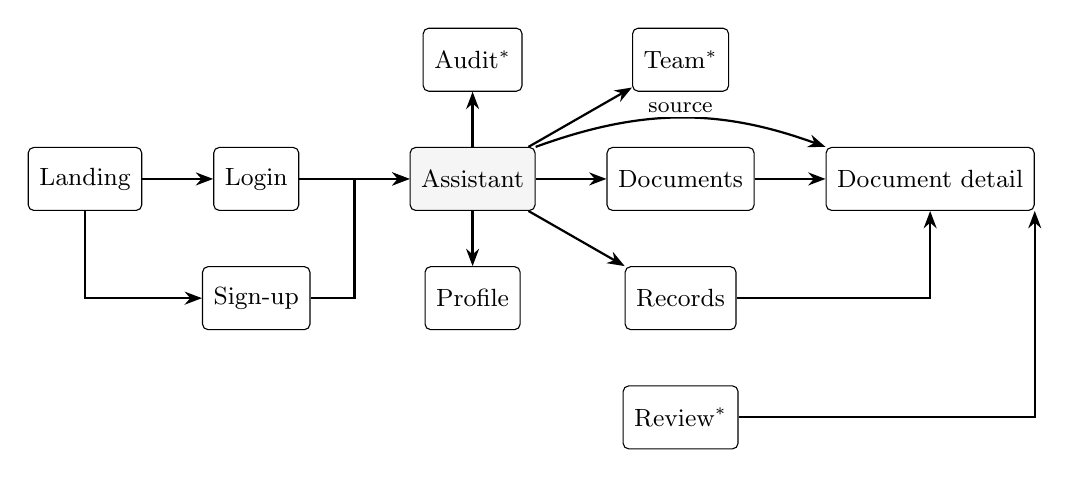
\begin{tikzpicture}[node distance=7mm and 9mm]
\node[box] (land) {Landing};
\node[box,right=of land] (login) {Login};
\node[box,below=of login] (reg) {Sign-up};
\node[box,right=14mm of login,fill=gray!8] (ask) {Assistant};
\node[box,right=of ask] (docs) {Documents};
\node[box,right=of docs] (det) {Document detail};
\node[box,below=of docs] (rec) {Records};
\node[box,below=of rec] (rev) {Review$^{\ast}$};
\node[box,above=of docs] (team) {Team$^{\ast}$};
\node[box,above=of ask] (aud) {Audit$^{\ast}$};
\node[box,below=of ask] (prof) {Profile};
\draw[flow] (land) -- (login);
\draw[flow] (land) |- (reg);
\draw[flow] (login) -- (ask);
\draw[flow] (reg) -| ($(login.east)!0.5!(ask.west)$) -- (ask);
\draw[flow] (ask) -- (docs);
\draw[flow] (docs) -- (det);
\draw[flow] (ask.north east) to[bend left=20] node[lbl,above]{source} (det.north west);
\draw[flow] (rec) -| (det);
\draw[flow] (rev) -| (det.south east);
\draw[flow] (ask) -- (aud);
\draw[flow] (ask) -- (prof);
\draw[flow] (ask) -- (team);
\draw[flow] (ask) -- (rec);
\end{tikzpicture}
\end{adjustbox}
\caption{Application Navigation Flow ($^{\ast}$ shown only to permitted roles)}\label{fig:navflow}
\end{figure}

\subsection{Responsiveness and Performance}
The frontend is built with Vite and loads each screen as a separate, lazily loaded bundle, so the first
page opens quickly. Heavy work (OCR, embeddings, model calls) never runs in the browser or in the
request that uploads a file; the interface polls the document status and updates when processing
finishes. The layout uses responsive breakpoints for laptop and tablet widths.

\section{Deployment}
\begin{table}[H]\centering
\caption{Deployment Details}\label{tab:deploy}
\begin{tabularx}{\textwidth}{|p{3cm}|X|}\hline
\textbf{Service} & \textbf{Configuration (docker-compose.yml)} \\ \hline
db & \code{pgvector/pgvector:pg16}, persistent volume, health check \\ \hline
backend & Python 3.12-slim image with Tesseract and CPU PyTorch; runs migrations and Gunicorn \\ \hline
worker & Same image; runs \code{python manage.py run\_worker} (processing and hourly reminders) \\ \hline
web & Node build of the Vue app served by Nginx, which also proxies \code{/api/} to the backend \\ \hline
Configuration & All secrets and provider settings in a \code{.env} file (never committed); \code{.env.example} documents every variable \\ \hline
\end{tabularx}
\end{table}
For development, the database runs in Docker while the API, worker and Vite dev server run locally.
A demonstration organization with users for every role and sample documents is created with
\code{python manage.py seed\_demo}.

\section{Chapter Summary}
This chapter described the development environment, the implementation of the six modules, the main
algorithms, the fine-tuning of the clause classifier, the external components, the user interface and
the deployment configuration. The next chapter tests and evaluates the system.

\chapter{Testing and Evaluation}
This chapter presents how \sysname{} was tested and how well its AI components perform. Testing
checks that the software does what the requirements say (unit, integration, system, performance and
security testing). Evaluation measures the quality of the AI components on public, expert-labelled
datasets, because an AI system can pass every functional test and still give wrong answers.

\section{Testing Strategy}
\begin{itemize}
\item \textbf{Unit and integration tests} are automated with Django's test framework and run with
\code{python manage.py test} against a temporary PostgreSQL database with pgvector. They run without any
LLM (the LLM is switched off in the test settings), so they are fast, free and repeatable; the language
model is evaluated separately.
\item \textbf{System (black-box) tests} exercise complete use cases through the user interface or its REST API.
\item \textbf{Performance tests} measure response and processing times on the development machine.
\item \textbf{Security tests} check authentication, the role $\times$ access-level matrix, file access and
the audit log.
\item \textbf{AI evaluation} uses CUAD~\cite{hendrycks2021cuad}, LEDGAR~\cite{tuggener2020ledgar}, a
labelled set of 100 routing questions and a handwriting set (Section~\ref{sec:eval}).
\end{itemize}

\section{Unit Testing}
All automated tests pass (34 tests, 97 seconds). Table~\ref{tab:unit} lists the unit tests.

\begin{longtable}{|p{1.15cm}|p{3.1cm}|p{4.1cm}|p{4.5cm}|p{1.2cm}|}
\caption{Unit Test Cases}\label{tab:unit}\\ \hline
\textbf{ID} & \textbf{Module / Function} & \textbf{Input} & \textbf{Expected Output} & \textbf{Result} \\ \hline
\endfirsthead
\hline
\textbf{ID} & \textbf{Module / Function} & \textbf{Input} & \textbf{Expected Output} & \textbf{Result} \\ \hline
\endhead
UT-01 & \code{parse\_date} & ``2025-03-12'', ``12th day of March, 2025'', ``March 12, 2025'', ``12/03/2025'', ``sometime next year'' & First four parse to 12 March 2025 (day-first); the last returns none & Pass \\ \hline
UT-02 & \code{ground} & Page ``The parties signed this agreement on 12 March 2025 in Lahore.''; a real and an invented quote & Real quote grounded; ``signed on 1 January 2020 in Karachi'' rejected & Pass \\ \hline
UT-03 & \code{chunk\_pages} & Two Contract Act pages with ``CHAPTER II'' and numbered sections 10 and 11 & Section 11 chunk starts on page 2 and its path contains ``CHAPTER II'' and ``11. Who are competent'' & Pass \\ \hline
UT-04 & \code{visible\_documents} & Every role $\times$ ORG / DEPARTMENT / RESTRICTED documents & Each user sees exactly the allowed set & Pass \\ \hline
UT-05 & Documents API & Employee of another department requests a department-only document & Not listed; detail and file return 404 & Pass \\ \hline
UT-06 & Documents API & Admin deletes a document & Document is archived (row kept) and disappears from other users' lists & Pass \\ \hline
UT-07 & \code{can\_edit} & Employee edits someone else's document & HTTP 403 & Pass \\ \hline
UT-08 & Upload permission & Auditor uploads a file & HTTP 403 & Pass \\ \hline
UT-09 & Upload validation & \code{virus.exe}; a \code{.pdf} file whose content is not a PDF & Both rejected with HTTP 400 & Pass \\ \hline
UT-10 & Versions \& compare & Upload version 2, compare with version 1 & Two versions kept; added and removed lines returned & Pass \\ \hline
UT-11 & Field correction & Manager corrects a field value & Value and status change; FieldEdit with old and new value & Pass \\ \hline
UT-12 & Verify permission & Employee verifies a field & HTTP 403 & Pass \\ \hline
UT-13 & AuditEvent & Update and delete an existing event & Both raise an error; event unchanged & Pass \\ \hline
UT-14 & \code{heuristic\_plan} & ``When was the NDA with Acme signed?'' & LOOKUP, field signed\_date, party Acme & Pass \\ \hline
UT-15 & \code{\_clean} & ``null'', `` None '', ``Acme'' & None, None, ``Acme'' & Pass \\ \hline
UT-16 & \code{heuristic\_plan} & ``Find the lease for the Lahore office''; ``What makes an agreement void under the law?'' & SEARCH; KNOWLEDGE & Pass \\ \hline
UT-17 & \code{answer} (lookup) & ``When was the NDA with Acme signed?'' & Answer contains ``12 March 2025''; source is the NDA & Pass \\ \hline
UT-18 & Ask API \& history & Two questions in one conversation; another user opens it & Conversation has 2 queries; other user gets 404 & Pass \\ \hline
UT-19 & \code{notice\_days} & ``thirty (30) days written notice'', ``60 days'', ``one month'', ``2 weeks'', ``reasonable notice'' & 30, 60, 30, 14, none & Pass \\ \hline
UT-20 & \code{run\_reminders} & Lease expiring in 25 days with 30 days' notice & ``expires in 25 days'' and ``notice deadline 5 days ago'' reminders, including for the admin & Pass \\ \hline
UT-21 & \code{run\_reminders} & Contracts expiring in 400 and 60 days; check run twice & No reminder for the far one; exactly one per person for the near one & Pass \\ \hline
UT-22 & \code{people\_to\_remind} & HR department-only contract expiring in 5 days & Admin and uploader notified; legal employee and outsider not & Pass \\ \hline
UT-23 & Notifications API & List and mark as read & Unread count drops to 0 & Pass \\ \hline
UT-24 & Streaming ask API & ``When was the NDA with Acme signed?'' & Events arrive as plan, sources, text, done; the text contains ``12 March 2025''; the question is saved to history & Pass \\ \hline
UT-25 & Streaming ask API & HR employee asks for the secret settlement codeword, passing its document id & No source from the forbidden document and none of its text in the stream & Pass \\ \hline
UT-26 & Answer cache & Same question asked twice by one user, then by a user with different access & Second answer comes from the cache; the other user gets a fresh answer & Pass \\ \hline
UT-27 & \code{confident\_search} & ``Find the lease \dots'', ``Show me all handwritten affidavits'', ``Show me the expiry dates \dots'' & First two skip the LLM routing call; requests naming a record field do not & Pass \\ \hline
UT-28 & \code{parse\_term} & ``three (3) years'', ``thirty-six months'', ``90 days'', ``until terminated'' & 36 months, 36 months, 90 days, none & Pass \\ \hline
UT-29 & \code{derive\_expiry} & Effective 1 April 2025, term ``3 years'', no written expiry & Expiry 31 March 2028, quote = the term, status NEEDS\_REVIEW & Pass \\ \hline
UT-30 & \code{derive\_expiry} & Same, but with a written expiry date & Written date kept, nothing calculated & Pass \\ \hline
UT-31 & Second check & Governing law (supported) and a notice period quoting a renewal clause (not supported) & Governing law stays AUTO; notice period goes to review with the reason & Pass \\ \hline
\end{longtable}

\section{Integration Testing}
Integration tests check that modules work together. IT-01, IT-03 and IT-04 are automated; IT-02, IT-05 and
IT-06 were run against the running system.

\begin{longtable}{|p{1.15cm}|p{3.4cm}|p{4.0cm}|p{4.4cm}|p{1.3cm}|}
\caption{Integration Testing Summary}\label{tab:integration}\\ \hline
\textbf{ID} & \textbf{Modules Integrated} & \textbf{Input} & \textbf{Expected Result} & \textbf{Result} \\ \hline
\endfirsthead
\hline
\textbf{ID} & \textbf{Modules Integrated} & \textbf{Input} & \textbf{Expected Result} & \textbf{Result} \\ \hline
\endhead
IT-01 & Upload API $\rightarrow$ job queue $\rightarrow$ extraction $\rightarrow$ chunking $\rightarrow$ embeddings $\rightarrow$ PostgreSQL & A generated multi-page PDF & Version READY; pages, chunks with embeddings and search vectors stored & Pass \\ \hline
IT-02 & Vue Assistant $\rightarrow$ Ask API $\rightarrow$ router $\rightarrow$ retrieval $\rightarrow$ LLM $\rightarrow$ viewer & ``When is a contract voidable under the Contract Act?'' on the 65-page Contract Act 1872 & Answer citing the Contract Act with pages; source opens the page & Pass (13.6\,s) \\ \hline
IT-03 & Access control $\rightarrow$ hybrid retrieval & A secret document visible only to the legal department; searches by an HR employee, an outsider and a legal employee & HR employee and outsider never receive its chunks; legal employee gets it first & Pass \\ \hline
IT-04 & Ask API $\rightarrow$ engine with explicit document ids & HR employee passes the secret document's id & Id ignored; no sources from it & Pass \\ \hline
IT-05 & LLM gateway $\rightarrow$ fallback provider & Main provider's daily quota exhausted (HTTP 429, retry after 20 min) & Gateway switches to the fallback at once and answers; later calls skip the main provider & Pass \\ \hline
IT-06 & Docker Compose: database, backend, worker, nginx web & \code{docker compose up} on an empty database, then \code{seed\_demo} & Migrations run; all four containers healthy; six documents processed; sign-in, lookup, streamed answer and protected file download work through nginx & Pass \\ \hline
\end{longtable}

\section{System Testing}
Black-box tests follow the use cases of Chapter~3, signed in as the demo users of each role. BB-08 to
BB-11 were run in the user interface; the others were run through the same REST API the interface calls,
using a script that only sees requests and responses (no access to the code or database). During BB-10 a
defect was found: for long passages, every short word of the passage was highlighted all over the page. The
viewer was changed to locate the passage as a whole in the page text, and the test was repeated.

\begin{longtable}{|p{1.15cm}|p{2.0cm}|p{4.6cm}|p{5.0cm}|p{1.3cm}|}
\caption{System (Black Box) Test Cases}\label{tab:blackbox}\\ \hline
\textbf{ID} & \textbf{Use Case} & \textbf{Steps} & \textbf{Expected Result} & \textbf{Result} \\ \hline
\endfirsthead
\hline
\textbf{ID} & \textbf{Use Case} & \textbf{Steps} & \textbf{Expected Result} & \textbf{Result} \\ \hline
\endhead
BB-01 & UC-1.1 Register & Register a new organization with its admin; sign in & Organization created (201); signed-in user has the Admin role & Pass \\ \hline
BB-02 & UC-1.2 Login & Sign in with a wrong, then the correct password & 401, then tokens issued; LOGIN events in the audit log & Pass \\ \hline
BB-03 & UC-1.3 Members & Admin creates HR and Legal departments, adds an HR Employee, uploads an organization-wide and a Legal-only document & Member created (201); the HR employee sees only the organization-wide document & Pass \\ \hline
BB-04 & UC-2.1 Upload & Upload an image-only (scanned) PDF and a handwritten page marked handwritten & Both READY (46 s and 6 s); pages read by OCR and by handwriting recognition & Pass \\ \hline
BB-05 & UC-2.2 Versions & Upload a lease, then version 2 with a new rent, and compare & Two versions listed; comparison shows the new rent & Pass \\ \hline
BB-06 & UC-3.1 Register & Filter the records register by ``lease'' & Only leases listed, with expiry dates (31 Dec 2026, 30 Jun 2027) & Pass \\ \hline
BB-07 & UC-3.2 Review & Manager corrects the first field in the review queue with a reason; Employee tries to verify & Field leaves the queue; history stores the reason; Employee gets 403 & Pass \\ \hline
BB-08 & UC-4.1 Lookup & Ask ``Which contracts expire in 2027?'' & Office lease listed with expiry 30 June 2027 and evidence & Pass (1.5\,s) \\ \hline
BB-09 & UC-4.2 Law book & Ask ``What does the Contract Act say about agreements without consideration?'' & Section 25 rule and its exceptions with citations & Pass \\ \hline
BB-10 & UC-4.3 Source & Open the first source of a Contract Act answer & Page 22 opens with only the cited passage highlighted (Figure~\ref{fig:scr-source}) & Pass \\ \hline
BB-11 & UC-4.4 History & Reopen an earlier conversation & Questions, answers and sources shown & Pass \\ \hline
BB-12 & UC-5.1 Audit & Download a file; Auditor filters the audit log by DOWNLOAD; Employee opens the audit log & Only DOWNLOAD events listed; Employee gets 403 & Pass \\ \hline
\end{longtable}

\section{Performance Testing}
Measurements were taken on the development laptop (CPU only) with the free tiers of the LLM providers.
During the measurement the main provider's daily token quota had been used by the evaluation runs, so
generated answers came from the fallback provider (Gemini).

\begin{table}[H]\centering
\caption{Performance Metrics}\label{tab:perf}
\begin{tabularx}{\textwidth}{|p{4.4cm}|p{3.2cm}|X|}\hline
\textbf{Metric} & \textbf{Requirement} & \textbf{Observed Result} \\ \hline
Lookup answer time & $\leq$ 3 s (PER-1) & 1.5 s (``Which contracts expire in 2027?'') \\ \hline
Knowledge answer time & $\leq$ 35 s (PER-2) & 11.5--13.6 s with a warm server; 22.8 s for the first question after a restart (model loading) \\ \hline
Streamed knowledge answer & -- & Sources shown after 2.6 s, first words after 4.1 s, complete after 4.4 s (Groq, warm server) \\ \hline
Upload response & Immediate (PER-3) & Returns after storing the file; processing continues in the background \\ \hline
Digital page extraction & -- & About 10 ms per page (65-page Contract Act read in 1.2 s) \\ \hline
Handwritten page reading & -- & 6.8 s for one handwritten receipt (vision model) \\ \hline
Classification / field extraction & -- & 1.1--1.8 s / 1.4--2.0 s per short document; 38.6 s per long CUAD contract \\ \hline
Chunking and embedding & -- & 0.1--0.2 s for 1--3 page documents; 26 s for the 65-page Contract Act (190 chunks, CPU) \\ \hline
Automated test suite & -- & 34 tests in 97 s \\ \hline
\end{tabularx}
\end{table}

\noindent\textbf{Observation.} On free LLM tiers the main limit is the provider's token quota, not the
system: when the quota was exhausted, answers first took up to 45 seconds while the system waited for
retries. The gateway was then changed to switch provider immediately when a provider reports a long
wait, and to skip that provider until its quota resets, which produced the times above (IT-05).

\section{Security Testing}
\begin{table}[H]\centering
\caption{Security Verification Summary}\label{tab:security}
\begin{tabularx}{\textwidth}{|p{4.5cm}|X|p{2.1cm}|}\hline
\textbf{Check} & \textbf{Method} & \textbf{Result} \\ \hline
Unauthenticated access & API calls without a token return 401 & Pass \\ \hline
Role $\times$ access-level matrix & UT-04 checks every role against every access level & Pass \\ \hline
Retrieval leakage & IT-03 / IT-04: forbidden chunks never returned, even when their ids are sent & Pass \\ \hline
File access & UT-05: files of invisible documents return 404 from the permission-checked endpoint & Pass \\ \hline
Privilege escalation & UT-07, UT-08, UT-12: edit, upload and verify blocked for the wrong roles & Pass \\ \hline
Audit integrity & UT-13: events cannot be updated or deleted & Pass \\ \hline
Password storage & Django PBKDF2 salted hashes; plain passwords never stored & Pass \\ \hline
Rate limiting & DRF throttling: 20 questions/min, 600 requests/hour per user & Configured \\ \hline
Secrets & API keys only in \code{.env}, which is git-ignored & Pass \\ \hline
\end{tabularx}
\end{table}

\section{AI Evaluation}\label{sec:eval}
The AI components were evaluated with scripts in \code{evaluation/} on public datasets labelled by
experts. Each experiment ID (EV-$n$) is referenced in the traceability matrix.

\subsection{EV-1: Clause Classification (LEDGAR)}\label{sec:eval-clauses}
Test set: 10,000 provisions, 100 clause types. Macro-F1 averages over all types, so rare types count as
much as common ones.

\begin{table}[H]\centering
\caption{Clause Classification Results on LEDGAR}\label{tab:ev-clauses}
\begin{tabularx}{\textwidth}{|X|r|r|r|r|}\hline
\textbf{Model} & \textbf{Training provisions} & \textbf{Test provisions} & \textbf{Accuracy} & \textbf{Macro-F1} \\ \hline
TF-IDF + logistic regression (baseline) & 10,000 & 10,000 & 81.7\% & 72.3\% \\ \hline
TF-IDF + logistic regression (baseline) & 60,000 & 10,000 & 87.7\% & 82.5\% \\ \hline
Fine-tuned all-MiniLM-L6-v2 (ours, CPU, 3 epochs) & 10,000 & 10,000 & 71.2\% & 45.9\% \\ \hline
Fine-tuned all-MiniLM-L6-v2 (ours, GPU, 5 epochs) & 60,000 & 10,000 & 85.1\% & 75.1\% \\ \hline
\textbf{Fine-tuned MiniLM + TF-IDF, averaged (ours, used by the system)} & \textbf{60,000} & \textbf{10,000} & \textbf{88.5\%} & \textbf{82.7\%} \\ \hline
Zero-shot LLM (\code{gpt-oss-120b}, no training) & 0 & 198 & 65.2\% & 44.0\% \\ \hline
\end{tabularx}
\end{table}

The zero-shot LLM was tested on a random sample of 198 test provisions because of the free-tier rate limit; 2 calls that failed at the API were excluded. It needs no training data, but with 100 closely related labels it is less accurate than both trained models, which supports fine-tuning a small local model for this task: it is also free and fast at inference time.

Training on all 60,000 provisions on a free Colab T4 GPU (13.2 minutes) raised the fine-tuned model from
71.2\% to 85.1\% accuracy and from 45.9\% to 75.1\% macro-F1; only 4 of the 100 clause types are still never
predicted. The laptop run had been under-trained: with 10,000 examples many rare classes had almost no
training data.

On its own, the fine-tuned model is still below the TF-IDF baseline. LEDGAR clause types are signalled
largely by vocabulary (``governing law'', ``indemnify''), which suits a keyword model, and MiniLM is a very
small encoder (22 million parameters) chosen for fast CPU inference. The two models, however, make different
mistakes: TF-IDF relies on exact wording, the transformer on meaning. The system therefore averages their
predicted probabilities (\code{ml/train\_ensemble.py}). The weight of the transformer (0.25) was chosen on
the 10,000 validation provisions only, and the test set was used once. In that run the combination reached
\textbf{88.5\% accuracy and 82.7\% macro-F1}, better than TF-IDF (87.8\% / 82.1\%) and the fine-tuned model
(85.1\% / 75.0\%) evaluated on the same test set. This combination labels clauses in the application. All
trained models clearly beat the zero-shot LLM (65.2\%), at no API cost.

\subsection{EV-2: Retrieval (CUAD)}
For 60 CUAD contracts, 344 questions were asked about clauses that lawyers had marked. A result is a
hit when the returned passage contains the lawyers' answer span. Two chunking methods and three
retrieval methods were compared (an ablation study).

\begin{table}[H]\centering
\caption{Retrieval Results on CUAD (60 contracts, 344 questions)}\label{tab:ev-retrieval}
\begin{tabularx}{\textwidth}{|X|l|r|r|r|r|}\hline
\textbf{Chunking} & \textbf{Retrieval} & \textbf{Hit@1} & \textbf{Hit@3} & \textbf{Hit@5} & \textbf{MRR@10} \\ \hline
Fixed 1,000 characters (v1) & Semantic only & 49.7\% & 72.4\% & 82.8\% & 0.634 \\ \hline
Fixed 1,000 characters (v1) & Keyword only & 49.4\% & 73.8\% & 84.3\% & 0.637 \\ \hline
Fixed 1,000 characters (v1) & Hybrid RRF & 61.3\% & 82.3\% & 88.7\% & 0.733 \\ \hline
Section-aware (ours) & Semantic only & 53.5\% & 77.0\% & 84.6\% & 0.668 \\ \hline
Section-aware (ours) & Keyword only & 51.7\% & 80.2\% & 85.8\% & 0.665 \\ \hline
\textbf{Section-aware (ours)} & \textbf{Hybrid RRF} & \textbf{61.6\%} & \textbf{86.0\%} & \textbf{93.0\%} & \textbf{0.746} \\ \hline
\end{tabularx}
\end{table}
Compared with the design of the first version (fixed chunks, semantic search only), the final design
raises Hit@1 from 49.7\% to 61.6\% and Hit@5 from 82.8\% to 93.0\%. Both changes help on their own:
hybrid retrieval adds about 10 points of Hit@1, and section-aware chunking adds about 4 points of Hit@5.

\subsection{EV-3: Record Field Extraction (CUAD)}
Forty CUAD contracts were processed by the extraction step (model \code{gpt-oss-20b}, 38.6 s per
contract). A prediction is correct when its quoted evidence overlaps the lawyers' span or its value
matches (same date, parties or jurisdiction).

\begin{table}[H]\centering
\caption{Field Extraction Results on CUAD (40 contracts)}\label{tab:ev-extract}
\begin{tabular}{|l|r|r|r|}\hline
\textbf{Field} & \textbf{Precision} & \textbf{Recall} & \textbf{F1} \\ \hline
Parties & 100.0\% & 100.0\% & 100.0\% \\ \hline
Signing date & 88.0\% & 59.5\% & 71.0\% \\ \hline
Effective date & 77.1\% & 84.4\% & 80.6\% \\ \hline
Expiry date & 100.0\% & 35.7\% & 52.6\% \\ \hline
Auto-renewal & 90.0\% & 56.2\% & 69.2\% \\ \hline
Notice period & 26.9\% & 70.0\% & 38.9\% \\ \hline
Governing law & 90.0\% & 77.1\% & 83.1\% \\ \hline
\textbf{All fields (micro)} & \textbf{80.7\%} & \textbf{71.7\%} & \textbf{75.9\%} \\ \hline
\end{tabular}
\end{table}
\begin{itemize}
\item \textbf{Evidence is real.} 175 of 176 quotes (99.4\%) were found word-for-word on the cited page,
so every value can be checked against its source.
\item \textbf{Label differences.} CUAD's \emph{Notice Period To Terminate Renewal} covers only notice to
stop a renewal, while our notice period is any termination notice, so many correct values count as false
positives. CUAD's \emph{Expiration Date} is often a duration (``continues for five years''), while the
system stores an explicit date only when one is written, which lowers recall.
\item \textbf{Limitation of the first review rule.} Only 2 of the 34 wrong predictions were sent to review,
because most wrong values carry a real quote that answers a slightly different question. Confidence and
grounding alone do not catch these. Two improvements address this (below).
\end{itemize}

\paragraph*{Improvement 1: a second check.} After extraction, one more LLM call is asked a narrower question for
each value: does this quote, on its own, prove the value \emph{as this field}? Values that fail go to the review
queue with the model's reason (e.g.\ ``the quote is about a cure period, not termination notice''). Run on the
same 176 saved predictions (\code{evaluation/eval\_verifier.py}, model \code{gpt-oss-20b}):

\begin{table}[H]\centering
\caption{Second Check on Extracted Values (176 predictions)}\label{tab:ev-verify}
\begin{tabular}{|l|r|r|}\hline
\textbf{Review rule} & \textbf{Wrong values flagged} & \textbf{Right values flagged} \\ \hline
Confidence and grounding only & 2 of 34 (5.9\%) & 7 of 142 (4.9\%) \\ \hline
\textbf{With the second check} & \textbf{11 of 34 (32.4\%)} & 17 of 142 (12.0\%) \\ \hline
\end{tabular}
\end{table}
The check catches more than five times as many wrong values, mostly notice periods whose quote was really
about a cure period or payment terms, at the cost of reviewers also confirming 10 more correct values. Several
of those are signing dates quoted from ``IN WITNESS WHEREOF \dots{} as of the date above'', a quote that indeed
does not contain the date, so checking them is reasonable. (The saved quotes are cut to 200 characters, so
inside the pipeline the check sees slightly more text.)

\paragraph*{Improvement 2: calculated expiry dates.} Many contracts state a term (``for three (3) years from the
Effective Date'') instead of an end date. When no end date is written, the system now calculates it from the
effective or signing date and the term (start + term $-$ 1 day), quotes the term as evidence and always sends
the value to review. A written expiry date is never replaced. The 30 contracts without a written expiry date
were extracted again and the expiry field was scored with and without the calculation on the same run
(\code{evaluation/eval\_expiry.py}):

\begin{table}[H]\centering
\caption{Expiry Date with and without the Calculation (40 contracts)}\label{tab:ev-expiry}
\begin{tabular}{|l|r|r|r|}\hline
\textbf{Expiry date} & \textbf{Precision} & \textbf{Recall} & \textbf{F1} \\ \hline
Written dates only & 100.0\% & 35.7\% & 52.6\% \\ \hline
\textbf{With calculated dates} & 94.7\% & \textbf{64.3\%} & \textbf{76.6\%} \\ \hline
\end{tabular}
\end{table}
Nine dates were calculated and eight were right; the wrong one belongs to a contract the lawyers marked as
having no fixed expiry, and like every calculated date it was sent to review.

\subsection{EV-4: Query Routing}
A set of 100 questions (40 LOOKUP, 35 KNOWLEDGE, 25 SEARCH) labelled by hand was routed by the keyword
rules and by the LLM router. ``Right field'' is the share of lookup questions for which the right record
field (e.g.\ signing date) was chosen.
\begin{table}[H]\centering\footnotesize
\caption{Query Routing Results (100 questions)}\label{tab:ev-router}
\begin{tabular}{|l|r|r|r|r|r|r|}\hline
\textbf{Router} & \textbf{Accuracy} & \textbf{Lookup F1} & \textbf{Knowl.\ F1} & \textbf{Search F1} & \textbf{Right field} & \textbf{Time} \\ \hline
Keyword rules (fallback) & 77.0\% & 74.0\% & 73.2\% & 88.9\% & 60.0\% & $<$1 ms \\ \hline
LLM router (\code{gpt-oss-20b}) & 94.0\% & 96.4\% & 94.4\% & 88.9\% & 100.0\% & 1163 ms \\ \hline
\end{tabular}
\end{table}
The LLM router is correct on 94 of 100 questions against 77 for the
keyword rules, and it chooses the right field for every lookup (100.0\% against
60.0\%). Every LOOKUP question was routed correctly; most remaining errors are
search requests treated as lookups or knowledge questions (2 and 3 of 25), which still
return the right documents as sources. During the run, 11 of the 100 calls hit the free-tier rate limit and were
answered by the keyword fallback, so the LLM figures are a slight underestimate. A routing call takes about
1.2 s.

\subsection{EV-5: Handwriting Recognition}
Character and word error rates (lower is better) on 30 pages (synthetic handwriting-style fonts) for Tesseract, the vision
model, and the pipeline's rule (vision model only when Tesseract is unsure). The pages were generated from handwriting-style fonts, which
are easier than real handwriting; the script \code{evaluation/eval\_handwriting.py --folder} repeats the test on real
scans with transcripts.
\begin{table}[H]\centering
\caption{Handwriting Recognition Results}\label{tab:ev-hand}
\begin{tabular}{|l|r|r|r|}\hline
\textbf{Reader} & \textbf{CER} & \textbf{WER} & \textbf{Time per page} \\ \hline
Tesseract OCR & 5.0\% & 17.2\% & 1.0 s \\ \hline
Vision-language model (\code{gemini/gemini-2.5-flash}) & 0.1\% & 0.4\% & 34.8 s$^{\ast}$ \\ \hline
Pipeline (5/30 pages sent to the vision model) & 2.6\% & -- & -- \\ \hline
\end{tabular}
\end{table}
Tesseract alone already reads these typed-looking ``handwriting'' fonts well (5.0\% character errors), while the
vision model is almost perfect (0.1\%). With the pipeline's rule, only the 5 pages where Tesseract was unsure were
sent to the vision model, which halves the error rate (2.6\%) while keeping most pages fast and free. Six vision
calls were refused by the free-tier rate limit; those pages are left out of the vision figures.
$^{\ast}$The vision time includes waiting for the rate limit; a single uncontended call took about 6--7 s
(Table~\ref{tab:perf}).


\subsection{EV-6: Answer Quality}
CUAD questions were asked through the full answer engine for 10 contracts: about 20 whose answer is in the
contract and 10 whose answer is not. Measures: answer judged correct against the lawyers' annotation,
citation hit rate, and abstention (saying ``not in the document'') when the clause is absent. Correctness is
graded by a second LLM call that sees the lawyers' annotation (LLM-as-judge). Both runs used Gemini
Flash-Lite, the system's configured fallback model, for answering and grading: a run with \code{gpt-oss-20b}
hit the free daily token limit part-way (19 of 31 answers were ``model unavailable'' messages), so it was not
used.

\paragraph*{Improving ``not in the document'' answers.} In the first run the model sometimes presented a related
clause as if it answered the question. The answering instructions were changed so that, when the sources do
not contain the answer, the reply must begin with ``The documents do not say'' and then mention what related
information they do contain, without presenting it as the answer. The automatic check for such replies was
also widened (it had missed wording such as ``no specific duration is explicitly stated''); with the wider
check alone, the first run already scores 9 of 10.

\begin{table}[H]\centering
\caption{Answer Quality Before and After the New Instructions}\label{tab:ev-answers}
\begin{tabular}{|l|r|r|}\hline
\textbf{Measure} & \textbf{Before} & \textbf{After (used)} \\ \hline
Correctly says ``not in the document'' when absent & 80.0\% (8/10) & \textbf{100.0\% (10/10)} \\ \hline
At least one citation contains the lawyers' span & 95.2\% & \textbf{100.0\%} \\ \hline
Answers that cite their sources & 100.0\% & 100.0\% \\ \hline
Wrongly says ``not in the document'' when present & 4.8\% (1/21) & 10.0\% (2/20) \\ \hline
Answer judged correct & 100.0\% & 85.0\% (17/20) \\ \hline
\end{tabular}
\end{table}
The new instructions make the system more careful: it no longer answers any question whose clause is absent,
and every answer cites the lawyers' passage. The price is two over-cautious replies in borderline cases (a
``minimum percentage'' clause for a \emph{Minimum Commitment} question, and a termination notice for a
non-renewal notice question), where the reply nevertheless quotes and cites the relevant clause. For a legal
records system an occasional over-cautious reply is safer than an invented answer, so the new instructions
are used. (One question in the second run failed because the provider was overloaded; it is counted as an
error, not as a wrong answer. A third, softer wording was also tried and rejected: it answered 4 of 10
absent-clause questions with related clauses.) Because the same model graded its own answers, the
correctness figures are estimates and should be read together with the citation hit rate, which is measured
directly against the lawyers' spans.

\section{Testing Summary}
\begin{table}[H]\centering
\caption{Test Summary}\label{tab:testsummary}
\begin{tabular}{|l|r|r|r|}\hline
\textbf{Test type} & \textbf{Cases} & \textbf{Passed} & \textbf{Failed} \\ \hline
Unit (automated) & 31 & 31 & 0 \\ \hline
Integration (3 automated, 3 manual) & 6 & 6 & 0 \\ \hline
System (black box) & 12 & 12 & 0 \\ \hline
Security checks & 9 & 9 & 0 \\ \hline
\end{tabular}
\end{table}
All automated unit and integration tests pass, and the security checks confirm that access rules hold at
every layer, including retrieval. The evaluation shows that the redesigned retrieval clearly outperforms
the first version's design and that extracted values are backed by real evidence, while it also
identifies honest limitations (a small clause model that does not yet beat a strong keyword baseline, and the review rule's blind spot)
that are discussed in the next chapter.

\chapter{Conclusion and Future Work}

\section{Conclusion}
\sysname{} was redesigned from a generic ``chat with your PDF'' tool into a legal records intelligence
system for organizations. It holds all of an organization's records in one shared repository protected
by role, department and named-person access rules applied before any retrieval; reads digital, scanned
and handwritten English documents; turns records into structured fields backed by verbatim evidence;
answers fact questions from the records table and explanation questions from long reference documents
such as the Contract Act 1872 with page citations; opens the source page for every answer; and keeps
query history, document versions, field-edit history and an append-only audit log. A clause classifier
was fine-tuned on LEDGAR, and every AI component was evaluated on public datasets. On CUAD, the final
retrieval design raised Hit@5 from 82.8\% to 93.0\% over the first version's design, and field
extraction reached a micro-F1 of 75.9\% with 99.4\% of evidence quotes found on the cited page.

\section{Limitations}
\begin{itemize}
\item The clause classifier reported here was trained on a laptop CPU with 10,000 examples and is
under-trained; the full GPU run is still to be reported.
\item Free LLM tiers limit throughput; heavy use falls back to a second provider or to passages only.
\item The review rule misses wrong values that carry a real but irrelevant quote.
\item English only; no native mobile application.
\end{itemize}

\section{Future Work}
\begin{itemize}
\item A second verification model that checks each extracted value against its field definition.
\item Urdu document and handwriting support.
\item A fully local deployment with an open-weight LLM for organizations that cannot use cloud APIs.
\item Clause-level comparison against a company's standard templates and risk flags.
\item Contract obligations tracking and calendar integration for reminders.
\end{itemize}


\clearpage
\phantomsection\addcontentsline{toc}{chapter}{Bibliography}
\begin{thebibliography}{99}
\bibitem{lewis2020rag} P. Lewis, E. Perez, A. Piktus, F. Petroni, V. Karpukhin, N. Goyal, H. K\"uttler, M. Lewis, W.-t. Yih, T. Rockt\"aschel, S. Riedel, and D. Kiela, ``Retrieval-augmented generation for knowledge-intensive NLP tasks,'' in \emph{Advances in Neural Information Processing Systems (NeurIPS)}, 2020.
\bibitem{hendrycks2021cuad} D. Hendrycks, C. Burns, A. Chen, and S. Ball, ``CUAD: An expert-annotated NLP dataset for legal contract review,'' in \emph{NeurIPS Datasets and Benchmarks Track}, 2021.
\bibitem{tuggener2020ledgar} D. Tuggener, P. von D\"aniken, T. Peetz, and M. Cieliebak, ``LEDGAR: A large-scale multi-label corpus for text classification of legal provisions in contracts,'' in \emph{Proc. LREC}, 2020.
\bibitem{chalkidis2022lexglue} I. Chalkidis, A. Jana, D. Hartung, M. Bommarito, I. Androutsopoulos, D. M. Katz, and N. Aletras, ``LexGLUE: A benchmark dataset for legal language understanding in English,'' in \emph{Proc. ACL}, 2022.
\bibitem{reimers2019sbert} N. Reimers and I. Gurevych, ``Sentence-BERT: Sentence embeddings using Siamese BERT-networks,'' in \emph{Proc. EMNLP-IJCNLP}, 2019.
\bibitem{wang2020minilm} W. Wang, F. Wei, L. Dong, H. Bao, N. Yang, and M. Zhou, ``MiniLM: Deep self-attention distillation for task-agnostic compression of pre-trained transformers,'' in \emph{NeurIPS}, 2020.
\bibitem{wolf2020transformers} T. Wolf \emph{et al.}, ``Transformers: State-of-the-art natural language processing,'' in \emph{Proc. EMNLP: System Demonstrations}, 2020.
\bibitem{malkov2018hnsw} Y. A. Malkov and D. A. Yashunin, ``Efficient and robust approximate nearest neighbor search using hierarchical navigable small world graphs,'' \emph{IEEE Trans. Pattern Analysis and Machine Intelligence}, vol. 42, no. 4, pp. 824--836, 2020.
\bibitem{cormack2009rrf} G. V. Cormack, C. L. A. Clarke, and S. Buettcher, ``Reciprocal rank fusion outperforms Condorcet and individual rank learning methods,'' in \emph{Proc. ACM SIGIR}, 2009.
\bibitem{smith2007tesseract} R. Smith, ``An overview of the Tesseract OCR engine,'' in \emph{Proc. ICDAR}, 2007.
\bibitem{sandhu1996rbac} R. S. Sandhu, E. J. Coyne, H. L. Feinstein, and C. E. Youman, ``Role-based access control models,'' \emph{IEEE Computer}, vol. 29, no. 2, pp. 38--47, 1996.
\bibitem{vue} Vue.js, ``The progressive JavaScript framework.'' [Online]. Available: https://vuejs.org
\bibitem{django} Django Software Foundation, ``Django.'' [Online]. Available: https://www.djangoproject.com
\bibitem{drf} Encode, ``Django REST framework.'' [Online]. Available: https://www.django-rest-framework.org
\bibitem{postgres} PostgreSQL Global Development Group, ``PostgreSQL.'' [Online]. Available: https://www.postgresql.org
\bibitem{pgvector} A. Kane, ``pgvector: Open-source vector similarity search for Postgres.'' [Online]. Available: https://github.com/pgvector/pgvector
\bibitem{chatpdf} ChatPDF. [Online]. Available: https://www.chatpdf.com
\bibitem{notebooklm} Google, ``NotebookLM.'' [Online]. Available: https://notebooklm.google
\bibitem{kira} Litera, ``Kira.'' [Online]. Available: https://www.litera.com/products/kira
\bibitem{luminance} Luminance. [Online]. Available: https://www.luminance.com
\bibitem{ironclad} Ironclad. [Online]. Available: https://ironcladapp.com
\end{thebibliography}


\appendix
\chapter{Source Code and Reproduction}
The source code is available at \url{https://github.com/Hammad-cue/documind_ai}.

\noindent Run the tests: \code{python manage.py test}\\
Create demo data: \code{python manage.py seed\_demo}\\
Train the clause classifier: \code{python ml/train\_clause\_classifier.py}\\
Run the evaluations and write the results: \code{python -m evaluation.run\_all} then \code{python -m evaluation.report}\\
Deploy: \code{docker compose up --build}


\end{document}
